\documentclass{statsoc}

\usepackage[a4paper]{geometry}
\usepackage{graphicx}
\usepackage[textwidth=8em,textsize=small]{todonotes}
\usepackage{amsmath}
\usepackage{amssymb}

\usepackage{natbib}
%\usepackage{caption}
%\usepackage{subcaption}
%\usepackage{subfigure}[caption=false]
\usepackage[caption=false]{subfig}
\newtheorem{theorem}{Theorem}
\newtheorem{assumption}{Assumption}
\newtheorem{lemma}{Lemma}
\newtheorem{corollary}{Corollary}
\usepackage{thm-restate}



\newcommand{\ba}{\boldsymbol{a}}
\newcommand{\bb}{\boldsymbol{b}}
\newcommand{\bc}{\boldsymbol{c}}
\newcommand{\bd}{\boldsymbol{d}}
\newcommand{\be}{\boldsymbol{e}}
\newcommand{\bff}{\boldsymbol{f}}
\newcommand{\bg}{\boldsymbol{g}}
\newcommand{\bh}{\boldsymbol{h}}
\newcommand{\bi}{\boldsymbol{i}}
\newcommand{\bj}{\boldsymbol{j}}
\newcommand{\bk}{\boldsymbol{k}}
\newcommand{\bl}{\boldsymbol{l}}
\newcommand{\bm}{\boldsymbol{m}}
\newcommand{\bn}{\boldsymbol{n}}
\newcommand{\bo}{\boldsymbol{o}}
\newcommand{\bp}{\boldsymbol{p}}
\newcommand{\bq}{\boldsymbol{q}}
\newcommand{\br}{\boldsymbol{r}}
\newcommand{\bs}{\boldsymbol{s}}
\newcommand{\bt}{\boldsymbol{t}}
\newcommand{\bu}{\boldsymbol{u}}
\newcommand{\bv}{\boldsymbol{v}}
\newcommand{\bw}{\boldsymbol{w}}
\newcommand{\bx}{\boldsymbol{x}}
\newcommand{\by}{\boldsymbol{y}}
\newcommand{\bz}{\boldsymbol{z}}
\newcommand{\bA}{\boldsymbol{A}}
\newcommand{\bB}{\boldsymbol{B}}
\newcommand{\bC}{\boldsymbol{C}}
\newcommand{\bD}{\boldsymbol{D}}
\newcommand{\bE}{\boldsymbol{E}}
\newcommand{\bF}{\boldsymbol{F}}
\newcommand{\bG}{\boldsymbol{G}}
\newcommand{\bH}{\boldsymbol{H}}
\newcommand{\bI}{\boldsymbol{I}}
\newcommand{\bJ}{\boldsymbol{J}}
\newcommand{\bK}{\boldsymbol{K}}
\newcommand{\bL}{\boldsymbol{L}}
\newcommand{\bM}{\boldsymbol{M}}
\newcommand{\bN}{\boldsymbol{N}}
\newcommand{\bO}{\boldsymbol{O}}
\newcommand{\bP}{\boldsymbol{P}}
\newcommand{\bQ}{\boldsymbol{Q}}
\newcommand{\bR}{\boldsymbol{R}}
\newcommand{\bS}{\boldsymbol{S}}
\newcommand{\bT}{\boldsymbol{T}}
\newcommand{\bU}{\boldsymbol{U}}
\newcommand{\bV}{\boldsymbol{V}}
\newcommand{\bW}{\boldsymbol{W}}
\newcommand{\bX}{\boldsymbol{X}}
\newcommand{\bY}{\boldsymbol{Y}}
\newcommand{\bZ}{\boldsymbol{Z}}
\newcommand{\balpha}{\boldsymbol{\alpha}}
\newcommand{\bbeta}{\boldsymbol{\beta}}
\newcommand{\bgamma}{\boldsymbol{\gamma}}
\newcommand{\bdelta}{\boldsymbol{\delta}}
\newcommand{\bepsilon}{\boldsymbol{\epsilon}}
\newcommand{\blambda}{\boldsymbol{\lambda}}
\newcommand{\bmu}{\boldsymbol{\mu}}
\newcommand{\bnu}{\boldsymbol{\nu}}
\newcommand{\bphi}{\boldsymbol{\phi}}
\newcommand{\bpi}{\boldsymbol{\pi}}
\newcommand{\bsigma}{\boldsymbol{\sigma}}
\newcommand{\btheta}{\boldsymbol{\theta}}
\newcommand{\bomega}{\boldsymbol{\omega}}
\newcommand{\bxi}{\boldsymbol{\xi}}
\newcommand{\bGamma}{\boldsymbol{\rho}}
\newcommand{\bDelta}{\boldsymbol{\Delta}}
\newcommand{\bTheta}{\boldsymbol{\Theta}}
\newcommand{\bLambda}{\boldsymbol{\Lambda}}
\newcommand{\bXi}{\boldsymbol{\Xi}}
\newcommand{\bPi}{\boldsymbol{\Pi}}
\newcommand{\bOmega}{\boldsymbol{\Omega}}
\newcommand{\bUpsilon}{\boldsymbol{\Upsilon}}
\newcommand{\bPhi}{\boldsymbol{\Phi}}
\newcommand{\bPsi}{\boldsymbol{\Psi}}
\newcommand{\bSigma}{\boldsymbol{\Sigma}}
\DeclareMathOperator*{\argmin}{arg\,min} 


\usepackage{comment}
\newcommand{\jx}[1]{{\color{blue}{ #1}}}
\newcommand{\ma}[1]{{\color{orange}{ #1}}}

\title[Broyden Quasi-Newton Acceleration for MM]{Quasi-Newton Acceleration of EM and MM Algorithms via Broyden's Method with Extrapolation}
\author[Medha Agarwal {\it et al.}]{Medha Agarwal}
\address{Department of Statistics, University of Washington, Seattle, U.S.A. }%\footnote{The work was completed when the author was an undergraduate student at Indian Institute of Technology Kanpur.}}
\email{medhaaga@uw.edu}
\author[Agarwal and Xu]{Jason Xu}
\address{Department of Statistical Science, Duke University,
Durham,
U.S.A.}
\email{jason.q.xu@duke.edu}



\begin{document}
\begin{abstract}

%In modern statistical computing, 
The principle of majorization-minimization (MM) provides a general framework for eliciting effective algorithms to solve optimization problems. However, they often suffer from slow convergence, especially in large-scale and  high-dimensional data settings. This has drawn attention to  acceleration schemes designed exclusively for MM algorithms, but  many existing designs are either  problem-specific or rely on approximations and heuristics loosely inspired by the optimization literature. We propose a novel, rigorous  quasi-Newton method for accelerating any valid MM algorithm, cast as seeking a fixed point of the MM \textit{algorithm map}. The method does not require specific information or computation from the objective function or its gradient, and enjoys a limited-memory variant amenable to efficient computation in high-dimensional settings. By connecting our approach to Broyden's classical root-finding methods, we establish convergence guarantees and identify conditions for linear and super-linear convergence. These results are validated numerically and compared to peer methods in a thorough empirical study, showing that it achieves state-of-the-art performance across a diverse range of problems.



\end{abstract}

\section{Introduction}
 Iterative procedures are becoming increasingly prevalent for statistical tasks that are cast as optimization of  objective functions lacking a closed form solution. The canonical setting of minimizing a measure of fit together with a penalty term sits at the heart of statistics, yet challenges still arise from high dimensionality, missing data, constraints, and other aspects of contemporary data. 
The principle of majorization-minimization (MM) provides a framework for designing effective algorithms well-suited for such problems. Perhaps the most well-known special case is the expectation-maximization (EM) algorithm, a workhorse for maximum likelihood estimation under missing data. The general MM principle is attractive because it admits algorithms that (1) are  simple to implement and (2) provide stable performance by obeying monotonicity in the objective  \citep{dempster1977maximum,laird1978nonparametric}.

However, MM algorithms typically converge at a locally linear rate, which can translate to impractically slow progress in many statistical problems, especially in high dimensions \citep{wu1983convergence,boyles1983convergence,meng1994global}. To address this issue,  a body of work designs general acceleration schemes for numerical optimization methods including Nesterov's schemes \citep{nesterov1983method}, SAG \citep{schmidt2017minimizing}, SAGA \citep{defazio2014saga}, catalyst acceleration \citep{lin2017generic}, and  SDCA \citep{shalev2014accelerated}. Special attention has also been given towards acceleration methods specifically designed for MM algorithms \citep{jamshidian1997acceleration, jamshidian1993conjugate, lange1995quasi, zhou2011quasi}. Broadly, these methods  seek additional information to better inform the search direction and/or step lengths of the unadorned algorithm. Improvements may come from high order differentials of the objective or  algorithm map that incur additional computational cost. Therefore, it becomes necessary to balance these tradeoffs.

So-called \textit{hybrid} accelerators  \citep{jamshidian1997acceleration} rely on working directly on the original objective function  \citep{lange1995quasi, jamshidian1997acceleration, jamshidian1993conjugate}. Approximate second order information can then be obtained via Fisher scoring in the case of EM. Outside of the context of missing data, classical tools such as quasi-Newton and conjugate gradient methods can be applied to the objective to similar effect. However, an advantage of MM algorithms lies in sidestepping unwieldy objectives in favor of operating on simpler surrogates---for instance, EM works well because it bypasses the need to consider the observed data log-likelihood. These hybrid methods unfortunately fail to preserve this key advantage of MM algorithms. %They would in fact be of limited use when it is nontrivial to evaluate the objective function or carry out its differentiation.

An alternative is to instead consider accelerating the MM algorithm map directly in a way that is largely agnostic to the optimization objective. These have been classified as \textit{pure} accelerators; see \cite{jamshidian1997acceleration}. One class of \textit{pure} first-order accelerators is given by quasi-Newton algorithms, which utilize approximate first-order information to find roots of the MM residuals. \cite{jamshidian1997acceleration} explicitly apply Broyden's classical root-finding algorithm for this purpose \citep{broyden1965class}. As we outlay our method, we will demonstrate that further improvement can be achieved by modifying a general Broyden-type method \citep{broyden1973local} that leverages extra information from the MM map. The STEM and SQUAREM methods of \cite{varadhan2008simple} approximate the Jacobian matrix of MM residuals by a scalar multiple of the identity matrix. The quasi-Newton method of \cite{zhou2011quasi} involves an assumption based on nearness to the stationary point, rendering it sensitive to initialization. These pure accelerators tend to preserve the simplicity, convergence properties, and low computational cost of the original algorithm. However, they often rely on heuristic approximations or derivations that potentially ignore a large amount of crucial first-order information. 
%As a result, they may suffer from ignoring a large amount of potentially crucial second-order information in practice. 
While loosely inspired by the theory behind classical quasi-Newton methods, it can be argued that these methods do not fully and formally take advantage of the prior optimization literature.


This paper seeks to fill the methodological gap by proposing a generic accelerator for any MM algorithm map $F$ via a quasi-Newton approximation to the Jacobian of the fixed point equation $G(x) = F(x) - x$.  We build off of the wisdom in \cite{zhou2011quasi}, referring to their  method as ZAL in this paper, that seeks a root of $G(x)$ without imposing positive definiteness constraints. Casting the problem in this way leads to robustness against numerical instabilities. Our method differs from ZAL in several important ways. While ZAL minimizes the norm of the Jacobian near the fixed point, we optimize a richer objective that directly ties into the classical approach of minimizing the change in the Jacobian across iterations. This standard quasi-Newton recipe demands storing the approximate Jacobian matrices in each iteration, which can be computationally ineffective for high dimensions. To address this issue, we further propose a limited-memory variant of our method amenable to high-dimensional settings. 

%We also show how our approach  can be seen as a unifying method generalizing several of the popular existing approaches above.. 



%The paper is organized as follows: Section 2 reviews majorization-minimization and quasi-Newton methods. Our proposed approach based on Broyden's method, beginning with an example that emphasizes how it differs from the standard version of Broyden's method is derived in Section 3. This section also presents a limited-memory variant of our approach and convergence analysis. In Section 4, these findings are validated empirically  on real and simulated data. The experiments comprise a conservative comparison against efficient implementations of the peer methods, focusing on problem settings considered in those preceding papers. We close with a brief discussion.

%While ZAL minimizes a simpler quantity, their choice yields the desirable property that iterates for Jacobian approximations only depend on the current state and the algorithm map. \ma{can also be states in the past; maybe also talk about how the objective tends to minimize the change in state rather than the change in H} The simpler structure of the updates makes it particularly amenable to high-dimensional settings, while storage costs may be overwhelming for our method when the number of variables may go up to an order of thousands or millions. To address this, we also propose a limited memory variant of our algorithm that significantly reduces the computation costs in high-dimensional cases. This is constructed in spirit of limited memory BFGS algorithm that ensures its numerical supremacy over other limited-memory algorithms (see \cite{liu1989limited}).   %(\cite{shanno1978conjugate}) and limited memory BFGS method (\cite{nocedal1980updating}). 

\section{Background: EM, MM, and Acceleration}


MM algorithms are increasingly popular toward  solving large-scale and high-dimensional optimization problems in statistics and machine learning \citep{lange2008mm, zhou2015novel,xu2019power}.
Consider $\bx \in \mathbb{R}^p$ and the goal of minimizing a ``difficult" objective function $f: \mathbb{R}^p \to \mathbb{R}$, i.e. of finding
$\displaystyle \bx^\ast = \text{argmin}_{\bx} f(\bx)\,. $ 
An MM algorithm transfers this task onto an iterative scheme, successively minimizing a sequence of surrogate functions $g(\bx \mid \bx_k)$ which dominate the objective function $f(\bx)$ and are tangent to it at the current iterate  $\bx_k$. %Decreasing $g(\bx \mid \bx_k)$  automatically engenders a decrease in $f(\bx)$, and a local optimum of $f(\bx)$ is found by successively minimizing the sequence of surrogates.  
%Majorization entails two conditions: tangency and domination. 
That is, they require  that $g(\bx_k \mid \bx_k) = f(\bx_k)$ and $g(\bx \mid \bx_k)  \geq f(\bx)$ for all $\bx$ at each iteration $k$. Decreasing $g(\bx \mid \bx_k)$  automatically engenders a decrease in $f(\bx)$.   The resulting update $\bx_{k+1}~=~\text{argmin}_{\bx} g(\bx \mid \bx_k)$ implies the string of inequalities
\begin{equation}\label{eq:descent}
  f(\bx_{k+1}) \leq g(\bx_{k+1} \mid \bx_{k}) \leq g(\bx_{k} \mid \bx_{k}) = f(\bx_{k}),
\end{equation}
validating the descent property. Examining this short proof of descent in Eq.\eqref{eq:descent} reveals that exact minimization of $g(\bx \mid \bx_k)$ is not strictly necessary, and any update that decreases $g$ is sufficient. A local optimum of $f(\bx)$ is found by successively minimizing the sequence of surrogates.   Our method will make use of this practically useful observation. 



The celebrated EM method for maximum likelihood estimation is a special case of this principle that relies on the notion of missing data to define the surrogate $g(\bx \mid \bx_k)$. Besides EM, instances of MM abound in statistics, ranging from matrix factorization \citep{lee1999learning} to nonconcave penalized likelihood estimation \citep{zou2008one}. 


The MM principle thus offers a general recipe for converting a hard optimization problem into a stable and simpler sequence of manageable subproblems, which can be expressed as an algorithm map in a $p$-dimensional space, denoted by $F$, that updates
\[
\bx_{k+1} = F(\bx_k).
\]
The iteration terminates when a chosen vector norm (usually $L_2$ norm) of differences between two consecutive iterates is small enough, i.e. $\|\Delta \bx_k\| = \|\bx_{k+1} - \bx_k\| \leq \epsilon$ for some tolerance $\epsilon > 0$. From the perspective of the algorithm map, the MM algorithm amounts to seeking the fixed point $\bx^\ast$ of $F$; an equivalent formulation that appears in the literature is to seek the root  of $G(\bx) := F(\bx) - \bx$. This approach has paved the way for quasi-Newton acceleration regimes that attempt to well-approximate the inverse of the Jacobian of $G$ at $\bx_k$; see \cite{luenberger1984linear, dennis1996numerical} for a more detailed discussion. Let $dG(\bx)$ be the differential of $G$ at $\bx$, then $dG(\bx) = (dF(\bx_k) - I_p)$ where $I_p$ is the $p \times p$ identity matrix. Denoting the approximation to $dG(\bx_k)^{-1}$ by $H_k$, the quasi-Newton update of $\bx_k$ is given by
\begin{equation}\label{eq:QN_update}
  \bx_{k+1} = \bx_k - H_k G(\bx_k)\,.  
\end{equation}
Various quasi-Newton methods differ from one another in the way $dG(\bx)^{-1}$ is approximated. The thread that ties them together is a \textit{secant condition}, which states that $H_k$ is the exact inverse Jacobian of a linear function joining $(\bx_k, G(\bx_k))$ and some other point of choice, say $(\by, G(\by))$. That is, the secant constraint mandates that $H_k$ satisfies
\begin{equation}\label{eq:sec}
\by - \bx_k = H_k (G(\by) - G(\bx_k))\,.
\end{equation}
In the classical Broyden's method, $\by$ is taken to be $\bx_{k+1}$ obtained using Eq.\eqref{eq:QN_update}, whereas \cite{zhou2011quasi} assume the function $G$ to be linear between the iterate $\bx_k$ and its image $ F(\bx_k)$ under the MM map. For $\bx  \in \mathbb{R}^p$,  $H_k$ is a $p \times p$ matrix and the secant constraint fixes $p$ degrees of freedom. The remaining $p^2 - p$ degrees entail that Eq.\eqref{eq:sec} is underdetermined, satisfied by infinitely many solutions $H_k$. At this juncture, deriving quasi-Newton methods proceeds by specifying an additional criterion to admit a well-defined procedure. We now survey various popular approaches along this line of thought.


%\jx{Briefly mention that there are multiple variants along this line of thought that exist, which we survey in the next section. In a sentence or two, describe what we want to do and at a very high level why it's different from existing methods as a transition}

\begin{comment}
\jx{What you have written here has lots of good information. Eventually we may split it up so that some references come in the introduction above, some contextualizes relations to existing work after we present our method, and the rest can become part a more specific background/literature review section to follow the introduction}.
\ma{We can possibly let go of this information. We can decide on one kind of classification and ignore giving a detailed overview of previous methods. This has been already done in many J&J and Varadhan & Roland papers.}
There has been wide discussion on methods for accelerating the EM algorithms in statistical community. \cite{varadhan2008simple} suggested a binary classification for EM accelerators - (1) monotone and (2) non-monotone acceleration schemes. Monotone accelerators target to increase the likelihood like EM algorithm. Prominent examples are parameter expansion EM (\cite{liu1998parameter}), Expectation Conditional Maximization (ECM) (\cite{meng1993maximum}), and ECME which shares the monotone convergence properties of EM and ECM while offering a faster convergence (\cite{liu1994ecme}). Non-monotone methods tend to find the root of an objective function, for example, $G(x) = F(x) - x$ where $F(x)$ is the fixed point algorithm map. These methods employ EM iterative schemes to get closer to the root of an objective function which gives the required maximum likelihood estimates. The most widely used and cited method for EM acceleration is the multivariate Aitken's acceleration suggested by \cite{louis1982finding}

\begin{equation}
    \Delta\theta_n = -(J - I)^{-1}g(\theta_n)
\end{equation}

where $\Delta \theta_n$ is the acceleration step, $g(\theta_n)$ is the current step and $J$ denotes the approximation to the Jacobian of the EM step. The method proposed by \cite{louis1982finding} to find $(J - I)$ is essentially the Newton Raphson method to find the zero of $g(x)$ (see discussion by \cite{laird1987maximum}; \cite{meilijson1989fast}). Other examples of monotone accelerators are conjugate gradient (CG) method (\cite{jamshidian1993conjugate}) and quasi Newton methods (\cite{jamshidian1997acceleration}; \cite{lange1995quasi}). The recent acceleration methods STEM and SQUAREM developed by \cite{varadhan2008simple} presents a different category which approximates the Newton's method using the idea of Steffenson's two point secant appoximation for the Jacobian. They build a vector form of this method for STEM and apply an idea of 'squaring' to obtain SQUAREM. \\

The monotone methods are fast and retain the ascent property of EM algorithms. However, they are highly dependent on the intrinsic model properties and hence cannot be broadly applied. Non-monotone methods are generally applicable but lack on the part of storage and globalised convergence. These methods store the Hessian of the algorithm map or require the observed information matrix which limits their use in high dimensional cases. They depend on the starting values and therefore, show poor results when started 'badly'. The SQUAREM requires only the algorithm map for EM and offer great results even for high dimensional problems. Following the work by \cite{varadhan2008simple}, \cite{zhou2011quasi}, built a quasi-Newton acceleration technique that retains the simplicity of SQUAREM. We will call this method ZAL (Zhou Alexander Lange) for future comparisons. As pointed out in \cite{zhou2011quasi}, we are interested in finding the root of the equation $F(x) - x = 0$ unlike the previous quasi Newton methods (\cite{jamshidian1997acceleration}; \cite{lange1995quasi}) that require optimization of the objective function. \\

Both SQUAREM and ZAL do not approximate the full Hessian for optimizing the objective function using Newton's method due to storage and computational complications. ZAL is based on the assumption that we start near the fixed point whereas SQUAREM is based on the assumption that the Jacobian is of the form $\alpha_n I_p$ where $\alpha_n$ is a scalar and $I_p$ is a p-dimensional identity matrix. 

\end{comment}

%[Transition into our method]

\subsection{Existing MM Acceleration Schemes} \label{sec:qn}

%\subsection{Prior work}

%\jx{describe the general idea of quasi newton and set up the constraints/objective specification} 
Perhaps the most transparent and well-studied quasi-Newton acceleration scheme was proposed by \cite{jamshidian1997acceleration}. Their method directly applies the quasi-Newton method for root finding by \cite{broyden1965class}, maintaining the inverse Jacobian approximation $H_k$ by the update
\[
\Delta H_k = \dfrac{(\Delta \bx_k - H_k \Delta G_k)\Delta \bx_k^T H_k}{\Delta \bx_k^T H_k \Delta \bx_k}\,,
\]
where $\Delta \bx_k = -H_k G(\bx_k)$, $\Delta G_k = G(\bx_k + \Delta \bx_{k}) - G(\bx_k)$, and $\Delta H_k = H_{k+1} - H_k$ for any time point $k$. Contributions since have noted that this dense matrix update becomes computationally prohibitive in high dimensions typical of contemporary data. The STEM method by \cite{varadhan2008simple} instead provides a simpler approximation of $H_k$ as only a scalar multiple of the identity matrix. Assuming $H_k = \alpha_k I_p$, three variants of STEM entail slightly different inverse Jacobian approximations under % by way of defining % inverse Jacobian approximations proposed for STEM method are 
\begin{equation} \label{eq:squarem_steplengths}
    \alpha_k^{(1)} = \dfrac{\bu_k^T \bv_k}{\bv_k^T \bv_k}, \qquad\qquad \alpha_k^{(2)} = \dfrac{\bu_k^T\bu_k}{\bu_k^T \bv_k}, \qquad\qquad \alpha_k^{(3)} = -\dfrac{ \|\bu_k\|}{\|\bv_k\|}\,,
\end{equation}
where 
$$\bu_k = F(\bx_k) - \bx_k, \quad \text{and} \quad \bv_k \, = \, G(F(\bx_k)) - G(\bx_k) \, = \,F^2(\bx_k) - 2F(\bx_k) + \bx_k.$$ The scalars $\alpha_k$ in \eqref{eq:squarem_steplengths} can be understood as various steplengths for each update rule. An extension to STEM known as SQUAREM was later proposed by the same authors \citep{varadhan2008simple}, using the idea of a ``squared" Cauchy method which may outperform traditional Cauchy methods. SQUAREM makes use of the following update
\[
\bx_{k+1} = \bx_k - 2\alpha_k\bu_k + \alpha_k^2\bv_k\,.
\] 
%\jx{to do: reword/reorganize transition to squareem} 
%The same steplength is used to arrive at the SQUAREM method. 
While SQUAREM outperforms many acceleration methods and is chiefly regarded for its simplicity, the loss of information due to the identity matrix approximation can remain severe, especially in high dimensional cases. 

 More recently, an acceleration scheme, referred to as ZAL, was proposed by \cite{zhou2011quasi}. It enjoys the same computational complexity as SQUAREM by avoiding matrix approximation of $dG(\bx_k)^{-1}$ in the quasi-Newton update formulation in Eq.\eqref{eq:QN_update} at each step, with update rule
\[
\bx_{k+1} = \bx_k - \left(I_p - \dfrac{\bv_k \bu_k^T}{\bu_k^T \bu_k} \right)^{-1} G(\bx_k) = (1 - c_k)F(\bx_k) + c_k F^2(\bx_k)
\]
where $c_k = \bu_k^T\bu_k/\bu_k^T\bv_k$ and the differences $\bu_k, 
\bv_k$ are as defined earlier. It is worth mentioning the secant constraint used in ZAL, as we will motivate a similar constraint in terms of the end points for our method in the next section. Let $M := dF(\bx^\ast)$. A key assumption made is that $\bx_k$ is close to the optimal point $\bx^\ast$ so that the following linear approximation is reasonable: 
%This secant approximation can be obtained by first order  Taylor expansion of the function $F$ centered at $\bx_k$. While the authors present the secant approximation in terms of the function $F$, we will write it in terms of its linear transformation $G$, where it is assumed to take a linear form between $\bx_k$ and $F(\bx_k)$, satisfying
\begin{equation} \label{eq:ZALsecant}
   F \circ F(\bx_k) - F(\bx_k) \approx M(F(\bx_k) - \bx_k)\,.   
\end{equation} 
As these methods too operate only with reference to the algorithm map, largely ignoring the objective function to be minimized, they will serve as comparisons for our proposed method. We next examine the merits of defining secant endpoints using  \eqref{eq:ZALsecant} within  Broyden's quasi-Newton paradigm in the following section. % begin through a simple illustrative example.



\section{A novel Broyden quasi-Newton method}


\paragraph{Illustrative Example.}
We begin by accelerating a classic MM example of minimizing the cosine function  $f(x) = \cos(x)$, using quasi-Newton to find the root of MM residual. The goal is to highlight the difference between our secant approximation made using end points in \eqref{eq:ZALsecant} and Broyden's standard method, providing concrete intuition on why the former approach improves performance. In particular, it shows explicitly how our approach leverages  information from the geometry of the MM map toward a nonlinear update. 
To derive a surrogate, consider the following quadratic expansion about $y \in \mathbb{R}$:
\begin{align*} 
\cos(x) \,& =\, \cos(y)-  \sin(y)(x -y)- \frac{1}{2}\cos(z)(x-y)^2 \\ \,&\, \leq  \cos(y) - \sin(y)(x - y) + \frac{1}{2}(x-y)^2
 \,\, :=\,\, g(x \mid y), 
 \end{align*}
where $z$ lies between $x,y$ and the inequality follows since $|\cos(z)|\leq 1$
\citep{lange2016mm}. Thus, $g(x \mid y)$ majorizes the original objective. It is straightforward to minimize $g$ and see that the resulting MM step is given by the nonlinear update formula
\[
x_{k+1} = F(x_k) = x_k + \sin(x_k)\,.
\]
We are interested in finding the root of $G(x) \,=\, F(x) - x \,=\, \sin(x)$. Consider a scenario in Figure~\ref{fig:secants}, where the previous and current iterates, labeled $A$ and $B$ respectively, lie on opposite sides of the root $x^\ast = \pi$ of the function $G$, denoted by the vertical dashed line. Let $C^\ast$ denote the next iterate obtained by the standard MM update from point $B$ without acceleration. 

\begin{figure}
    \centering
    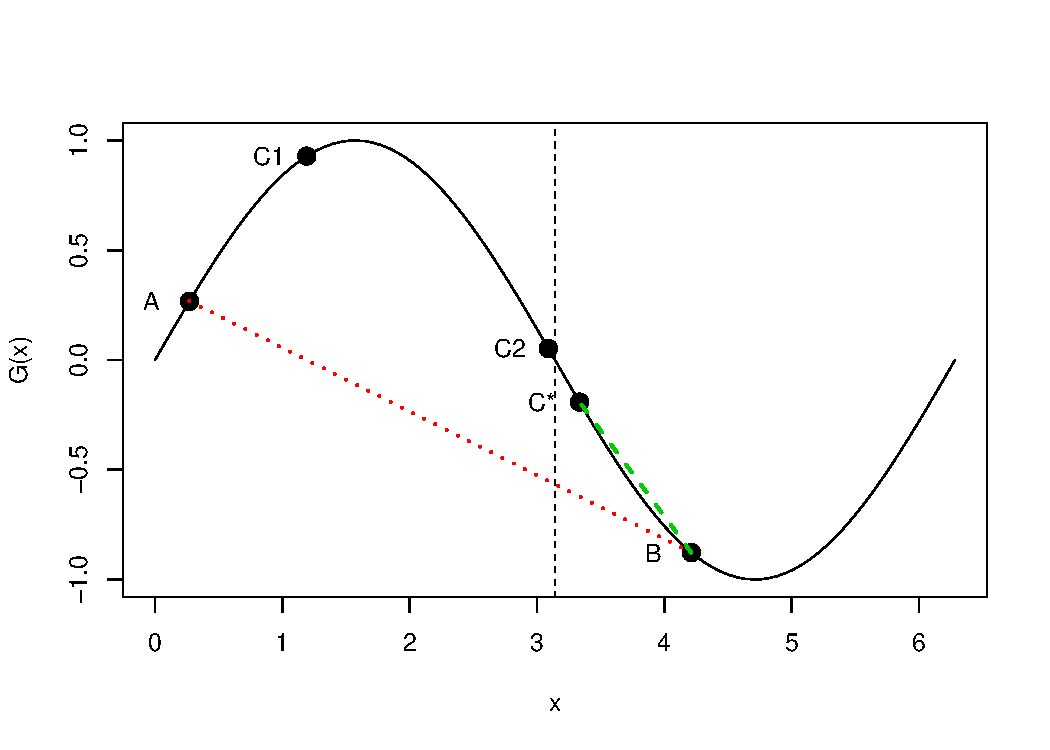
\includegraphics[width = .7\textwidth]{plots/secants.pdf}
    \caption{Comparison of secant approximations.}
    \label{fig:secants}
\end{figure}
Rather than moving to $C^\ast$, the standard Broyden's method approximates the Newton search direction as the slope of the line joining A and B (dotted red), whereas our update derived below will use the line joining $B$ and $C^*$ as the search direction (dashed green). As a result, the next iterate from standard Broyden's method would yield $C_1$ whereas our update, described in the next section, leads to $C_2$, much closer to the optimum. Denoting the corresponding points on the $x$-axes as $a, b, c^*, c_1,$ and $c_2$, the formulation for both the updates is
\[
c_1 = b - G(b)\dfrac{b - a}{G(b) - G(a)} \qquad \text{and} \qquad c_2 = b - G(b)\dfrac{c^* - b}{G(c^*) - G(b)}\,.
\]

Even in a univariate setting, where $H_k$ can be completely determined from the secant condition, the advantage provided by our novel secant approximation is clear when the current state does not render a good search direction. The additional information  can act as a correction when the original algorithm leads us to a \textit{bad} current state (here $B$). Because the secants drawn in the standard version of Broyden's method rely only linearly on the current and previous state, a bad quasi-Newton step propagates to a poor secant approximation that produces an update straying far from the fixed point. Our proposed method avoids this by drawing a secant that incorporates information at the current state together with an extrapolation from the next MM step, as we detail below. While this example would have been trivial to optimize directly, it illustrates an advantage that tends to become more pronounced in higher dimensions where the added directional information we harness from the MM extrapolation is richer.
 


\paragraph{Deriving the proposed method.}
Recall that seeking the fixed points of the MM map amounts to finding the roots of  $G(\bx)$ numerically. The quasi-Newton update is given by Eq.\eqref{eq:QN_update}. Drawing inspiration from the secant approximation in \eqref{eq:ZALsecant}, we propose the linear approximation
\begin{equation} \label{eq:secant_approx}
    dG(\bx_k)^{-1} \left[G(F(\bx_k)) - G(\bx_k)\right] \approx F(\bx_k) - \bx_k\,.
\end{equation}
Using the differences $\bu_k, \bv_k$ as introduced in the previous section and recalling $H_k$ denotes the approximation to $dG(\bx_k)^{-1}$ that satisfies \eqref{eq:secant_approx}, the secant condition can be expressed as $H_{k}\bv_k = \bu_k$. Note that one may impose several secant approximations $H_k (\bv_k^i) = \bu_k^i$ for $i \in \{1, ..., q\}$ for any choice such that $q < p$. These can be generated at the current iterate $\bx_k$ and previous $(q-1)$ iterates, and may yield better performance at the cost of extra computation. To this end, let $U_k = (\bu_1\;\bu_2 \dots \bu_q)$ and $V_k = (\bv_1 \; \bv_2 \dots \bv_q)$ be two $\ p\times q$ matrices; the corresponding linear constraint for $H_k$ in the multiple secant conditions case is
\begin{equation} \label{eq:bqn_secant_condition}
    H_k V_k = U_k\,.
\end{equation}
The $p \times p$ inverse Jacobian matrix $H_k$ has $p^2$ degrees of freedom, of which $pq$ degrees of freedom are fixed by the secant approximation. To derive a well-defined update, one must choose how to fix the remaining $p^2 - pq$ degrees of freedom. We follow classical intuitions that yield a connection to Broyden's method for finding roots of nonlinear functions.  
The idea behind this and several of the most successful quasi-Newton methods seeks the smallest perturbation to $H_{k-1}$ when updating to $H_k$, which can also be viewed as imposing a degree of smoothness in the sequence of iterates. The resulting optimization problem can be formulated as
\begin{align} \label{eq:minimization}
    \text{Minimize} &: \|H_{k} - H_{k-1}\|_F\,  \nonumber\\
    \text{subject to} &: H_{k}V_k = U_k\;,
\end{align} 
where $\|\cdot\|_F$ denotes the Frobenius norm. To proceed, we take  partial derivatives of the Lagrangian
\[
\mathcal{L} = \dfrac{1}{2}\|H_{k} - H_{k-1}\|^2_F + \Lambda^T(H_{k}V_k - U_k)
\]
with respect to $h_{k}^{ij}$ and set to ${0}$. Here $h_{k}^{ij}$ denotes the $ij^{th}$ element of the matrix $H_{k}$. As a consequence, we obtain the Lagrange multiplier equation
\[
0 = h_{k}^{ij} - h_{k-1}^{ij} + \sum_{k=1}^{p}\lambda_{ik}v_{jk},
\]
which can be expressed in matrix form as
\begin{equation} \label{eq:legrange_eq1}
H_{k} - H_{k-1} + \Lambda V_k^T = \mathbf{0}   .
\end{equation}
Right-multiplying Eq.\eqref{eq:legrange_eq1} by $V_k$ and imposing the constraint from Eq.\eqref{eq:bqn_secant_condition} gives the solution for $\Lambda$ as
\[
     \Lambda = (H_{k-1} V_k - U_k)(V_k^TV_k)^{-1}\,.
\]
Therefore, 
\begin{equation}
H_{k} = H_{k-1}\left(I_p - V_k (V_k^T V_k)^{-1}V_k^T\right) + U_k(V_k^T V_k)^{-1}V_k^T.
\end{equation}
We remark that as the problem dimension increases, a larger choice of $q$ fixes more information and may improve acceleration, but also risks numerical singularity for the matrix $V_k^T V_k$. We draw attention to the special case of $q=1$ where % is the most successful  where:
\begin{equation} \label{eq:BFGS_update}
    H_{k} = H_{k-1} - H_{k-1}\dfrac{\bv_k\bv_k^T}{\bv_k^T\bv_k} + \dfrac{\bu_k\bv_k^T}{\bv_k^T\bv_k}\,.
\end{equation}
We see \eqref{eq:BFGS_update} can be written as $H_{k} = H_{k-1} + A_k + B_k$ where both $A_k$ and $B_k$ are rank-1 matrices, yielding a rank-2 update as expected. Also note that the symmetry condition on $H_k$ assumed in classical Broyden-Fletcher-Goldfarb-Shanno (BFGS) updates for minimization is \textit{not} necessary, as here we are approximating an inverse Jacobian  rather than a Hessian/inverse Hessian matrix.

The search direction $\bp_k$ at iteration $k$ is given by $\bp_k = -H_{k}G(\bx_k)$, with a corrected update formula $\bx_{k+1} = \bx_k + \gamma_k \bp_k$, where $\gamma_k = \omega_k /\|\bp_k\|$ is an appropriate scaling factor in the search direction. Here $\omega_k$ is the steplength and $\|\cdot\|$ denotes the $L_2$ vector norm. The corresponding steplength for the unaccelerated MM algorithm is $\|F(\bx_k) - \bx_k\| = \|\bu_k\|$, and for a SQUAREM algorithm is $|\alpha_k^{(i)}| \|\bu_k\|$ for $i \in \{1,2,3\}$. We choose the steplength $|\alpha_k^{(3)}| \|\bu_k\| = \|\bu_k\|^2/\|\bv_k\|$ from \eqref{eq:squarem_steplengths} for our experiments in this paper due to its intuitive explanation \citep{varadhan2008simple}. %Suppose we use the steplength $\|H_k\| \|G(\bx_k)\|$ in the search direction $p_k = -H_k G(\bx_k)$. If $H_k$ is sufficiently close to $H_{k+1}$, Eq.\eqref{eq:ZALapprox} allows us to bound $\|H_k\|$ below by $\|\bu_k\|/\|\bv_k\|$. This bound guides a practical steplength rule given by $\alpha_k = \|\bu_k\|^2/\|\bv_k\|$. Note that this $\alpha_k$ coincides with the third version of SQUAREM. 
While the behavior of each of the three variants of SQUAREM varies widely, we will see that our method in contrast performs consistently well in a range of scenarios fixing  $\omega_k =\|\bu_k\|^2/\|\bv_k\|$.


%corresponding to the first and second steplengths of SQUAREM. In this paper, we will only focus on the $\alpha_t$ explicitly mentioned above. 



\paragraph{Intuition and relation to existing methods.} 
 
%Broyden's classic quasi-Newton method and its  variants \citep{schubert1970modification, klement2014using} remain a current state-of-the-art for numerically finding roots of a non-linear functions. The goal in Broyden's quasi-Newton method is to approximate the Jacobian of $G(.)$ at the current iterate $\bx_k$ by a linear approximation of $G(.)$ between $\bx_k$ and $\bx_{k-1}$. 
ZAL and SQUAREM are perhaps the most widely used quasi-Newton acceleration methods for MM algorithms. The point of departure in these methods is to cast acceleration as seeking a zero of $G$. We delve a little further into the connection between quasi-Newton root-finding methods and MM acceleration; in particular, we ground our approach in the wisdom behind Broyden's method, and improve upon it by designing a novel secant approximation with endpoints as $\bx_k$ and $F(\bx_k)$. As illustrated in the demonstrative example, the benefits of this extrapolation step are twofold. By the descent property of the MM map, $F(\bx_k) - \bx_k$ gives a more reliable direction to move along, % from $x_k$, $x_k - \bx_{k-1}$, 
especially when $\bx_k$ was a  poor update from $\bx_{k-1}$. Second, instead of only one constraint, the MM map enables us to impose multiple linear constraints that become increasingly accurate as iterates $\bx_k$ approaches $\bx^\ast$. %The idea of better secants enabled by MM algorithm can be seen in the demonstrative example below. 

In contrast, the STEM and SQUAREM methods employ scalar multiples of the identity as approximations to the Jacobian matrix, which can ignore much valuable curvature information compared to a dense approximation. % to the  which despite being computationally tempting, causes immense loss of information. 
Unlike traditional root finders for non-linear functionals \citep{broyden1965class, pearson1969variable}, their convergence properties are not as rigorously established. The ZAL method makes an assumption that $\bx_k$ is close to the stationary point $\bx^\ast$, validating the linear approximation in Eq.\eqref{eq:ZALsecant}. If $M_k$ denotes the approximation to $dF(\bx^\ast)$ at step $k$, then using the principle of parsimony, the objective in ZAL seeks to minimize $\|M_k\|_F$  subject to the constraint $V_k = (M_k - I_p)U_k$. This criterion yields a computationally elegant update, but unlike Eq.\eqref{eq:minimization} for BQN, effects a disconnect from the theory and intuition behind quasi-Newton methods based on minimally perturbing $H_k$, i.e. Eq. \eqref{eq:minimization}. It is unclear %whether this QN method will converge to the root of $G(.)$ function 
how convergence is affected when initiated far from a stationary point where the linear approximation is not reasonably valid. It is our understanding that this approach may fail or converge slowly in such cases, %, if at all, when the starting point is located sufficiently far away from the stationary point
since penalizing $M_k$ discourages large steps even when the current estimate is far from stationarity. % by the minimization condition. 
%\jx{may soften the claim at the end here}.

It can be argued that 
%the choice of cruder Jacobian approximations is made in light of computational considerations---  
a chief advantage of these prior methods is their computational simplicity. In particular, they are quite scalable to high-dimensional problems as their space complexity only grows linearly in the number of variables.
While bringing us closer to established optimization theory, our method produces Jacobians that may become computationally unwieldy as the number of variables grows. To ameliorate this,  we next propose a low-memory variant  based on the ideas in limited-memory BFGS. 
%The following section presents a version toward matching the computational merits of existing approaches while preserving our core idea.
%Whereas the design of ZAL and SQUAREM methods is more immediately applicable in such scenarios. To resolve this problem, at least on a comparative scale, we propose a limited memory version of our; algorithm that follows the idea limited memory BFGS.

\subsection{A limited memory variant for high-dimensional settings} 
Examining Eq.\eqref{eq:BFGS_update} reveals that our algorithm requires the $p \times p$ matrix $H_{k}$ to perform a rank-two update at each step, which can be computationally prohibitive in high dimensions. Additionally, storing the full $p \times p$ matrix at each step can be very challenging. Fortunately, many limited memory variants of  quasi-Newton algorithms have been proposed \citep{shanno1978conjugate,nocedal1980updating,griewank1982partitioned}, and rooting our method in Broyden's  framework allows us to immediately import these ideas. 

We will construct the limited memory version of our algorithm denoted by L-BQN by analogy to the way BFGS algorithm is made scalable using L-BFGS \citep{liu1989limited}. BFGS \citep{fletcher2013practical} is a quasi-Newton optimization method that stores an approximation of the inverse Hessian matrix of the objective function at each iteration. For computationally challenging high-dimensional cases, L-BFGS surpasses this problem by instead storing only a few vectors that represent the inverse Hessian approximation implicitly. Likewise, we will also store a pre-defined $m$ number of vectors that will approximate the inverse Jacobian at each step. Recall that our update is given by $\bx_{k+1} = \bx_k - H_k G(\bx_k)$, where $H_{k}$ is updated by the formula
\[
    H_{k+1} \quad=\quad H_{k}\left(I_p - \dfrac{\bv_k \bv_k^T}{\bv_k^T \bv_k}\right) + \dfrac{\bu_k \bv_k^T}{\bv_k^T \bv_k} \quad=\quad H_k W_k +\dfrac{\bu_k \bv_k^T}{\bv_k^T \bv_k},
\]
where $W_k = \left( I- \bv_k \bv_k^T/\bv_k^T \bv_k\right)$. Akin to the L-BFGS method, we may store $m$ previous pairs of $\{\bu_i, \bv_i\}$, $i = k-1, \dots , k-m$, where $m$ typically is chosen between $3$ and $20$. The matrix product required at each step $H_k G(\bx_k)$ can be obtained by performing a sequence of inner products and vector summations involving only $G(\bx_k)$ and the pairs $\{\bu_i, \bv_i\}$, $i = k, \dots, k-m$. After the new iterate is computed, the oldest pair $\{\bu_{(k-m)}, \bv_{(k-m)}\}$ is dropped and replaced by the pair $\{\bu_{k+1}, \bv_{k+1}\}$ obtained from the current step. %In this way, the set of vector pairs encodes curvature information using the $m$ most recent iterations.


A limited memory variant proceeds by recursion  at each iteration. At the  $k^{th}$ step, an initial estimate of the inverse Jacobian is taken to be a scalar multiple of identity matrix  $H_k^0= \nu_kI_p$. The scale factor $\nu_k$  attempts to capture the size of the true inverse Jacobian matrix along the most recent search direction. %In contrast to standard BFGS, $H_k^0$ is allowed to vary across iterations by updating $\nu_k$ at each  step. 
Next,  $H_k^0$ is updated $(m+1)$ times via Eq.\eqref{eq:BFGS_update} in a nested manner to obtain the relation
\begin{align*}
    H_{k} \; &= \; H_k^0 (W_{k-m} \ldots W_{k}) + \dfrac{\bu_{k-m} \bv_{k-m}^T}{\bv_{k-m}^T \bv_{k-m}}(W_{k-m+1} \ldots W_{k})\\
            \; & \quad + \; \dfrac{\bu_{k-m+1} \bv_{k-m+1}^T}{\bv_{k-m+1}^T \bv_{k-m+1}} (W_{k-m+2} \ldots W_{k}) + \; \ldots
            + \; \dfrac{\bu_{k} \bv_{k}^T}{\bv_{k}^T \bv_{k }}\,.
\end{align*}
Details on obtaining the nested formula above can be found in Chapter 6 of \cite{nocedal2006numerical}. There the authors suggest that an effective choice for the scaling factor is given by $ \nu_k = {\bu_{k}^T \bv_{k}}/{\bv_{k}^T \bv_{k}}.$
Through this choice, our L-BQN algorithm can be understood as a generalization of the STEM method \citep{varadhan2008simple}: STEM corresponds to the special case where $m=0$. However,  the approximate inverse Jacobian  $\nu_k I_p$ for STEM is derived by minimizing the distance between the zeros of two linear secant-like approximations for $G(\bx)$--- one centered around $\bx_k$, and another at $F(\bx_k)$. While the approaches that lead to this approximation are quite different, it accords more confidence in L-BQN as for non-zero $m$, the inverse Jacobian approximation is made \textit{more} robust by leveraging curvature information from the last $m$ iterates. % instead of being approximated by a scalar multiple of the identity matrix using just the last iterate. 
%Now that we have presented our acceleration method, we will provide convergence results in the next section. 



\subsection{Convergence}
We now analyze the convergence properties of the proposed method.
The two essential components %for the convergence recipe 
are \, 1) convergence of the base MM algorithm to the stationary point $\bx^\ast$, and \, 2) convergence of Broyden's root finding quasi-Newton method to the stationary point $\bx^\ast$ of the map $G$. Our study bridges careful analyses of these two facets. %Studying the nature of these two convergence, we can construct the collective proof of convergence for our algorithm.
%Typically, MM algorithms exhibit a locally linear rate of convergence \citep{lange2016mm}. 

Naturally, establishing convergence guarantees for our proposed acceleration scheme  rests on the convergence of the underlying MM map, which typically exhibits a locally linear rate of convergence \citep{lange2016mm}. We will assume the base algorithm to be locally convergent in a neighborhood $S$ of $\bx^\ast$ with  rate of convergence denoted by $\tau > 0$. In this section, we prove that BQN is also locally convergent to $\bx^\ast$ in a subset of this neighborhood, and further identify conditions that establish its convergence rate. 
Recall  $\{\bx_k\}$ converges to $\bx^\ast$ at a \textit{linear} rate if, for some chosen vector norm $\|\cdot\|$,
\[
\dfrac{\|\bx_{k+1} - \bx^\ast\|}{\|\bx_k - \bx^\ast\|} \leq r
\]
for some rate of convergence $r \in (0,1)$. The convergence rate is \textit{superlinear} if 
\[
\dfrac{\|\bx_{k+1} - \bx^\ast\|}{\|\bx_k - \bx^\ast\|} \to 0 \qquad\text{ as } k \to \infty\,.
\]
%Intuitively, the convergence of our MM acceleration method fundamentally banks on the convergence of the underlying MM algorithm map. We require the MM algorithm to be locally convergent, i.e. the algorithm converges to optimum value $\bx^\ast$ if we start in a neighborhood of the limit point, to guarantee the validity of our primary optimization method. 

%In this section, we have proved that given local convergence of MM algorithm in a neighborhood, our acceleration method is locally convergent to the limit point in a subset of this neighborhood. 

A seminal work of \cite{broyden1973local} derives  local linear and $Q$-superlinear convergence results for several single and double rank quasi-Newton root finding methods. % under  reasonable assumptions. %based on Broyden's approach of updating Jacobians. 
Our approach stands close to Broyden's second method, %\citep{broyden1965class}, 
while the improved secant approximation through  MM extrapolation will be incorporated into the analysis. We assume that $G$ is differentiable in a neighborhood of $\bx^\ast$, in that the Jacobian matrix $dG(\bx^\ast)$ exists and is non-singular. At many instances, we will treat $(\bx, dG(\bx)^{-1})$ as a tuple whose individual components are updated via Eq.\eqref{eq:QN_update} and \eqref{eq:BFGS_update}. It is crucial to prove that the update function in Eq.\eqref{eq:QN_update} is well defined in some neighborhood of the limit point $(\bx^\ast, dG(\bx^\ast)^{-1})$. To this end, we first prove by induction local convergence of our algorithm under certain conditions. We then carefully construct a neighborhood of $(\bx^\ast, dG(\bx^\ast)^{-1})$ to satisfy these conditions explicitly. 

To ease notation, our current iterate is denoted by $(\bx,H)$ in a neighborhood of $(\bx^\ast, dG(\bx^\ast)^{-1})$. We use $\bar{\bx}$ to denote the update on $\bx$ given by Eq.\eqref{eq:QN_update}, $\bar{H}$ to denote the update on $H$ from Eq.\eqref{eq:BFGS_update}, and introduce further notations: % for the following differences 
$$\bs = \bar{\bx} - \bx,\, \quad \by = G(\bar{\bx}) - G(\bx), \quad  \bu = F(\bx) - \bx, \quad \text{and} \quad \bv = G(F(\bx)) - G(\bx). $$
In the subsequent discussion, suppose $\|\cdot\|$ denotes a chosen vector norm on $\mathbb{R}^p$, then for a $p \times p$ matrix $A$, $\|A\|$ denotes the corresponding induced operator norm. The lemma below supplies useful inequalities to be applied in proving the main theorem. 

\begin{lemma} \label{lemma:lipchitz}
Assume $G: \mathbb{R}^p \to \mathbb{R}^p$ is differentiable in the open convex set $D$, and suppose that for some $\widehat{\bx}$ in $D$ and $d > 0$,
\begin{equation} \label{eq:lipchitz}
    \|dG(\bx) - dG(\widehat{\bx})\| \leq K \|\bx-\widehat{\bx}\|^d\,,
\end{equation}
where $K \in \mathbb{R}$ is a constant. Assuming $dG(\widehat{\bx})$ is invertible, we have for each $\by, \bz $ in $D$,
\begin{align}
    \|G(\by) - G(\bz) - dG(\widehat{\bx})(\by-\bz)\| & \leq K \max\{\|\by - \widehat{\bx}\|^d, \|\bz - \widehat{\bx}\|^d\}\|\by-\bz\| \label{eq:ineq1}  \nonumber \\
    \|dG(\widehat{\bx})^{-1}(G(\by) - G(\bz)) - (\by - \bz)\| &\leq K \|dG(\widehat{\bx})^{-1}\| \max\{\|\by - \widehat{\bx}\|^d, \|\bz - \widehat{\bx}\|^d\} \|\by-\bz\|\,.
\end{align}
%\end{subequations} 
 Moreover, there exists $\epsilon >0 \text{ and } \rho >0$ such that 
 \[ \max\{\|\by - \widehat{\bx}\|^d, \|\bz - \widehat{\bx}\|^d\} < \epsilon\] 
 implies that $\by \text{ and } \bz$ belong to $D$, and
\begin{equation} \label{eq:ineq2}
    (1/\rho)\|\by-\bz\| \leq \|G(\by) - G(\bz)\| \leq \rho\|\by-\bz\|\,.
\end{equation}
\end{lemma}
Inequalities (\ref{eq:ineq1}) follow from standard arguments using Taylor's expansion \citep{ortega2000iterative}, while inequality (\ref{eq:ineq2}) is an immediate consequence of continuity and non-singularity of $dG$ at $\widehat{\bx}$. In the subsequent analysis, we will use a matrix norm $\|\cdot\|_M$, not related to the vector norm $\|\cdot\|$ described earlier. Here, $\|A\|_M := \|MAM\|_F$ where $M$ is a matrix and $\|\cdot\|_F$ is the Frobenius norm. However, there is a constant $\eta > 0$ such that $\|A\| \leq \eta \|A\|_M$ by the equivalence of norms in finite-dimensional vector spaces. 

We now derive general sufficient conditions for local convergence in the spirit of a classic result  by \cite{broyden1973local}. Since we require the inverse of $dG$, we posit the following conditions before proving convergence, with $S \text{ and } D$ as defined earlier.
%Next we show that our proposed acceleration method satisfies these conditions, thus achieving the convergence result.

\begin{assumption} \label{ass1}
(A1) Let the function $G: \mathbb{R}^p \to \mathbb{R}^p$ be differentiable in the open convex set $D$ containing $\bx^\ast$ such that $G(\bx^\ast)=0$ and $dG(\bx^\ast)$ is non-singular. Assume that for some $d > 0$, $G$ satisfies Inequality~\eqref{eq:lipchitz} inside $D$.
\end{assumption}

\begin{assumption} \label{ass2}
(A2) %Firstly, we introduce the notation $N_1$ and $N_2$ for the neighborhoods of $\bx^\ast$ and $dG(\bx^\ast)^{-1}$ that are key to this assumption. 
Let the update function in Eq.\eqref{eq:QN_update} be well-defined in a neighborhood $N1$ of $\bx^\ast$ where $N_1 \subset D \cap S$, and inverse Jacobian update from Eq.\eqref{eq:BFGS_update} be well-defined in a neighborhood $N_2$ of $dG(\bx^\ast)^{-1}$ containing non-singular matrices. Assume that there are non-negative constants $\alpha_1 \text{ and } \alpha_2$ such that for each tuple $(\bx,H)$ in $N1 \times N2$, the following is satisfied,
\begin{align} 
    \|\bar{H} - dG(\bx^\ast)^{-1}\|_M &\leq \left[1 + \alpha_1 \max\left\{\|F(\bx) - \bx^\ast\|^d, \|\bx - \bx^\ast\|^d\right\}\right]\|H - dG(\bx^\ast)^{-1}\|_M \nonumber \\
    & \quad + \alpha_2 \max\left\{\|F(\bx) - \bx^\ast\|^d, \|\bx-\bx^\ast\|^d\right\} \label{eq:jacobian_error}\,.
\end{align}
\end{assumption}
The first assumption warrants the application of Lemma~\ref{lemma:lipchitz} on $G$, and the second assumption lends a key error bound on the inverse Jacobian estimation. The notion of well-defined used in Assumption~\ref{ass2} will be qualified for BQN later in Theorem~\ref{th:qnm_convergence}. 

\begin{theorem} \label{th:convergence}
Let A\ref{ass1} hold true for the function $G$ and A\ref{ass2} be satisfied for some neighborhoods $N_1$ and $N_2$ and non-negative constants $\alpha_1 \text{ and } \alpha_2$. Then for each $r \in (0,1)$ there exist positive constants $\epsilon(r) \text{ and } \delta(r)$ such that   the sequence with $\bx_{k+1} = \bx_k - H_kG(\bx_k)$ is well-defined and converges to $\bx^\ast$ whenever $\|\bx_0 - \bx^\ast\| < \epsilon(r)$ and $\|H_0 - dG(\bx^\ast)^{-1}\|_M < \delta(r)$. Furthermore,
\[
\|\bx_{k+1} - \bx^\ast\| \leq r\|\bx_k - \bx^\ast\| \qquad \text{ for each } k \geq 0,
\]
and the sequences $\{\|H_k\|\}$ and $\{\|H_{k}^{-1}\|\}$ are uniformly bounded.
\end{theorem}
A detailed proof appears is in the Appendix. %, which extends the argument outlined by Broyden to our context without strengthening the necessary assumptions. 
Under Theorem 1, we inherit the following property by an identical argument of \citet{broyden1973local}, with proof omitted here.

\begin{corollary} \label{cor:superlinear_conv}
Assume that the conditions of Theorem~\ref{th:convergence} hold. If some subsequence of $\{\|H_k - dG(\bx^\ast)^{-1}\|_M\}$ converges to zero, then $\{\bx_k\}$ converges Q-superlinearly to $\bx^\ast$.
\end{corollary}
%\begin{proof}
%The proof follows the technique used for proving Q-superlinearity of classical Broyden's method \cite[see Corollary 3.3]{broyden1973local}, so it is omitted here.
%\end{proof}

%Having specified the conditions required for local and $Q$-superlinear convergence, 
It remains to show that our acceleration algorithm satisfies the assumptions of Theorem \ref{th:convergence} and Corollary~\ref{cor:superlinear_conv}. The following result and subsequent corollary identify concrete conditions on the update functions $F \text{ and } G$ that ensure this. %the assumptions of Theorem~\ref{th:convergence} are met. 


\begin{theorem} \label{th:qnm_convergence}
Let A\ref{ass1} hold true for the function $G
$. If 
\begin{equation} \label{eq:ineq3}
    \dfrac{\|M\bv - M^{-1}\bv\|}{\|M^{-1}\bv\|} \leq \mu_2\|\bv\|^p,\qquad \bv \neq 0\,,
\end{equation}
for a constant $\mu_2 \geq 0$, non-singular and symmetric matrix $M \in \mathbb{R}^{p \times p}$, and all $(\bx, H)$ in a neighborhood $N^\prime$ of $(\bx^\ast, dG(\bx^\ast)^{-1})$, then the update functions \eqref{eq:BFGS_update} is well-defined in a neighborhood $N$ of $(\bx^\ast, dG(\bx^\ast)^{-1})$ and the corresponding iteration
\[
\bx_{k+1} = \bx_k - H_kG(\bx_k)
\]
is locally convergent to the limit point $\bx^\ast$. 
\end{theorem}
We emphasize that this result does not require stronger conditions than those imposed in the classical results pertaining to Broyden acceleration, %%\cite{broyden1973local}, 
which have endured as  reasonable mild assumptions in the optimization literature. 
\begin{corollary} \label{cor:q-superlinear}
If further $\displaystyle \lim_{k \to \infty}\|\bx_{k+1} - F(\bx_k)\|/\|\bx_k - \bx^\ast\| = 0$ holds, then the convergence rate of $\{ \bx_k \} $ to $\bx^\ast$ is Q-superlinear.
\end{corollary}
The complete technical proofs of these results are detailed in the Appendix.

\section{Results and Empirical Performance} \label{subsec:BFGSex}

We now turn to a  performance assessment %of our proposed acceleration algorithm 
on a variety of real and simulated data examples, including (a) quadratic minimization using Landweber's method, (b) maximum likelihood estimation in a truncated beta-binomial model, (c) the largest (and smallest) eigenvalue problem for symmetric matrices, and (d) location-scale estimation of a multivariate $t$-distribution. % together pose diverse challenges and exhibit the breadth of application. 
These problems were selected as examples in the prior studies that introduced the competing methods we benchmark against, thus offering a conservative comparison.
%together they pose diverse challenges and exhibit the breadth of application.  
As peer methods, we consider (1) unaccelerated MM, (2) the ZAL accelerator, %with $q = 2$ secant conditions,
(3) the three variants of SQUAREM, and (4) our proposed BQN method as well as (5) its limited memory variant L-BQN.

All methods are implemented using \texttt{R}; we use the implementation of  ZAL and SQUAREM in the \texttt{R} package \texttt{turboEM}.  Throughout our examples, we use the first-order ($K=1$) scheme for SQUAREM as proposed by \cite{varadhan2008simple} as the standard of comparison, since the $K=2$ and $K=3$ schemes are deemed less reliable  by the original authors. The implementation of the proposed accelerators, BQN and L-BQN, and all data examples are implemented as an \texttt{R} package \texttt{quasiNewtonMM} \footnote{\texttt{https://github.com/medhaaga/quasiNewtonMM}}. We consider $q=1$ and $q=2$ secant conditions for the proposed method as well ZAL. %It is noteworthy that our method as well as  ZAL as implemented by its authors uses \texttt{R}, while the \texttt{SQUAREM} package has an optimized implementation that calls subroutines implemented in lower level languages. For leveled comparison, we refrain from using the \texttt{SQUAREM} package.
%except for when the history of all iterates until convergence is required for plotting (Example 3) since \texttt{turboEM} package does not deliver that as a function output. 
%That BQN often outperforms  and remains competitive  in terms of runtime despite its naive implementation, unlike the other accelerators in \texttt{turboEM} package, attests to its efficacy. For ZAL, we restrict ourselves to $q=1$ and $q=2$ comparisons, in line with the number of secant conditions used for BQN. 


Stopping criteria are matched across all methods, declaring convergence at $\bx^\ast$ when $\|F(\bx^\ast) - \bx^\ast\| \leq \epsilon$ for a specified tolerance $\epsilon$. For ZAL and BQN, we revert to the original MM step whenever updates violate monotonicity, following \citet{zhou2011quasi}. In most cases,
we observe that BQN performs strikingly well and at least on par with its competitors. An overall theme is that existing methods may outpace our approach on some examples but then falter on a case-by-case basis, while BQN succeeds consistently. %At other times, BQN performs as well as the other aforementioned acceleration algorithms. 

%For each example, we attempt to minimize the objective like negative log-likelihood or mean-square error. 

\subsection{Landweber's method for quadratic minimization}

%\jx{If we do derive some theory and we assume conditions such as Lipschitz, then we may move this example up first and say that it is meant to confirm the theory in practice, i.e. we observe superlinear rate compared to the unaccelerated algorithm}.

\begin{table}

\caption{\label{tab:quadratic} Quadratic minimization of $f(\theta) = \theta^T A \theta/2 + b^T \theta$ for $100$ random starting points. 
}
\centering

\fbox{\begin{tabular}{c c c c } 
 \hline
 Algorithm & $F$ evals  & Time (in sec) & Objective \\ [0.5ex] 
 \hline
 
 MM & 194872.5 (179472.5, 207076.8)  & 4.218 (3.870, 4.470)  & -24.0591 (-24.0591, -24.0591) \\
 BQN, $q=1$ & 5724.0 (4719.5, 6510.0)  & 0.400 (0.330, 0.450) & -24.0602 (-24.0612, -24.0596) \\
 BQN, $q=2$ & 2953.0 (2616.5, 3501.0)   & 0.226 (0.196, 0.274)  & -24.0604 (-24.0614, -24.0599)   \\
 L-BQN & 12856.0 (11260.0, 13772.5)  & 0.631 (0.562, 0.698)  & -24.0592 (-24.0598, -24.0591)   \\
 SqS1 & 2150.0 (1926.5, 2412.0)  & 0.140 (0.127, 0.156) & -24.1067 (-24.1081, -24.1052)\\
 SqS2 & 12665.0 (11515.5, 13855.0)  & 0.833 (0.745, 0.909) & -24.0974 (-24.0983, -24.0968) \\
 SqS3 & 5911.0 (5092.0, 6374.5) & 0.410 (0.348, 0.445)  & -24.1062 (-24.1064, -24.1060)   \\
 ZAL & 23015.50 (21638.25, 24150.75)  & 1.655 (1.544, 1.741) & -24.1081 (-24.1081, -24.1080)  \\[1ex] 
%  MM & 138677.5 (123277.5, 150881.8)  & 7.127 (6.209, 7.691)  & -24.0591 (-24.0591, -24.0591) \\
%  BQN, $q=1$ & 4001.0 (3311.0, 4757.0)  & 0.642 (0.527, 0.781) & -24.0608 (-24.0622, -24.0596) \\
%  BQN, $q=2$ & 2170.0 (1900.0, 2637.5)  & 0.389 (0.335, 0.488)  & -24.0605 (-24.0612, -24.0600)  \\
%  L-BQN & 9230.50  (7922.75, 10121.75)  & 1.049 (0.887, 1.150)  & -24.0592 (-24.0594, -24.0591)   \\
%  SqS1 & 1718.0 (1414.0, 2034.5)  & 0.278 (0.224, 0.336) & -24.1068 (-24.1079, -24.1054)\\
%  SqS2 & 4197.0 (3589.0, 4773.5)  & 0.693 (0.583, 0.801) & -24.1062 (-24.1064, -24.1060) \\
%  SqS3 & 4197.0 (3589.0, 4773.5) & 0.690 (0.601, 0.781)  & -24.1062 (-24.1064, -24.1060)   \\
%  ZAL & 17909.5 (16536.0, 19042.5)  & 2.805 (2.589, 2.975) & -24.1081 (-24.1081, -24.1080)  \\[1ex] 
 \hline
 
\end{tabular}}
\end{table}
We begin with the ``well-behaved" problem of minimizing a quadratic function $f: \mathbb{R}^p \to \mathbb{R}$ using an MM iterative scheme. For $\theta \in \mathbb{R}^p$, consider a quadratic objective function
\[
f(\theta) = \dfrac{1}{2}\theta^T A \theta + b^T \theta\,,
\]
where $A$ is a $p \times p$ positive definite matrix and $b \in \mathbb{R}^p$. The exact solution is available by solving the linear equation $A\theta = -b$, but incurs a complexity of $\mathcal{O}(p^3)$.
  To avoid this computational cost, Landweber's method instead effects an iterative scheme, making use of the Lipschitz property of gradient of $f(\theta)$. The method can be viewed from the lens of majorization-minimization  \citep{lange2016mm}: since $\nabla f(\theta) = A \theta + b$, we can write the gradient inequality
%
\[
\|\nabla f(\theta) - \nabla f(\Phi)\| = \|A(\theta - \Phi)\| \leq \|A\|\|\theta - \Phi\| .
\]
%
As a consequence, the spectral norm of A is the Lipschitz constant for $\nabla f(\theta)$. Let the constant $L > \|A\|$. Landweber's method gives the following majorization for $f(\theta)$:
%
\begin{align*}
    f(\theta) \leq f(\Phi) + \nabla f(\Phi)^T (\theta - \Phi) + \dfrac{L}{2}\|\theta - \Phi\|^2 .
\end{align*}
Minimizing the above surrogate function then yields the MM update formula
\[
\theta_{n+1} = \theta_n - \dfrac{1}{L}\nabla f(\theta_n) = \theta_n - \dfrac{1}{L}(A\theta_n + b) .
\]
%The goal is to show that in high dimensions, standard MM algorithm might be very slow. 
Consider the problem dimension to be $p=100$ and tolerance to be $\epsilon = 10^{-5}$. We use a randomly generated $A$ and $b$ such that at true minima, the value of objective function is $-24.10846$. Due to the simple structure of the optimization problem, we might expect all algorithms to perform reasonably well, while we already see the unaccelerated MM algorithm converges very slowly.  % As $p$ increases, finding minima using MM algorithm gets increasingly computationally prohibitive. Therefore, we employ different quasi-Newton acceleration methods discussed in previous sections and compare their performance to our proposed algorithm. 
Table~\ref{tab:quadratic} reports performance in terms of the median and (interquartile range), comparing the number of $F$ function evaluations ($F$ evals), wall-clock time, and objective values at convergence over $100$ random initializations centered at the true mean, perturbing each component by normal noise with variance $1000$. Figure~\ref{fig:quad_boxplot} displays runtime and function evaluations as boxplots for BQN with $q=1$ (B1), BQN with $q=2$ (B2), L-BQN (L-B), SQUAREM-3, and ZAL. Initial values are matched across methods for each trial.   %initial guess for $100$ different replications. 
%Each method 
%We report three quantiles - $0.25,\,0.50,\text{ and } 0.75$ in the form $0.50 \,(0.25, 0.75)$ from these $100$ randomly generated starting values with mean at the true minimum and variance of $1000 \times I_{100}$, where $I_{100}$ is the $(100 \times 100)$ identity matrix. 
Given the strongly convex objective, all methods successfully deliver the minimum here. 

Our proposed BQN method with $q=1$ performs on par with the default SQUAREM-3, while using  $q=2$ secant conditions provides further  improvement. However, we notice that SQUAREM-1 outpaces our method in this case. This may be unsurprising as this ``easy" problem is favorable to methods that do not need to fully utilize curvature information, but are simple and fast. 
It is also worth noting that the variations of SQUAREM already perform quite differently from one another, suggesting significant  sensitivity to the choice of step-length. As mentioned earlier, the performance of ZAL tends to depend on the starting point, and we observe it tends to converge more slowly in this case when initialized with large perturbations of the true value.  
%Out of the three SQUAREM versions, we plot only for SQUAREM-3 because of two reasons - 1) it is deemed as default method by the authors in the \texttt{SQAUREM} \texttt{R} package, and 2) the chosen steplength of BQN matches the third version of SQUAREM steplengths, thus making it closest to our method for leveled comparisons.


%Performance in this example suggests that the limited-memory variant of our method as well as ZAL may not be worth choosing over their simpler counterparts, though they all improve upon the vanilla MM algorithm by orders of magnitude.



 %Notice that ZAL method consistently requires more F evaluations as well as time for convergence. 

\begin{figure}[!htbp]
    \centering
    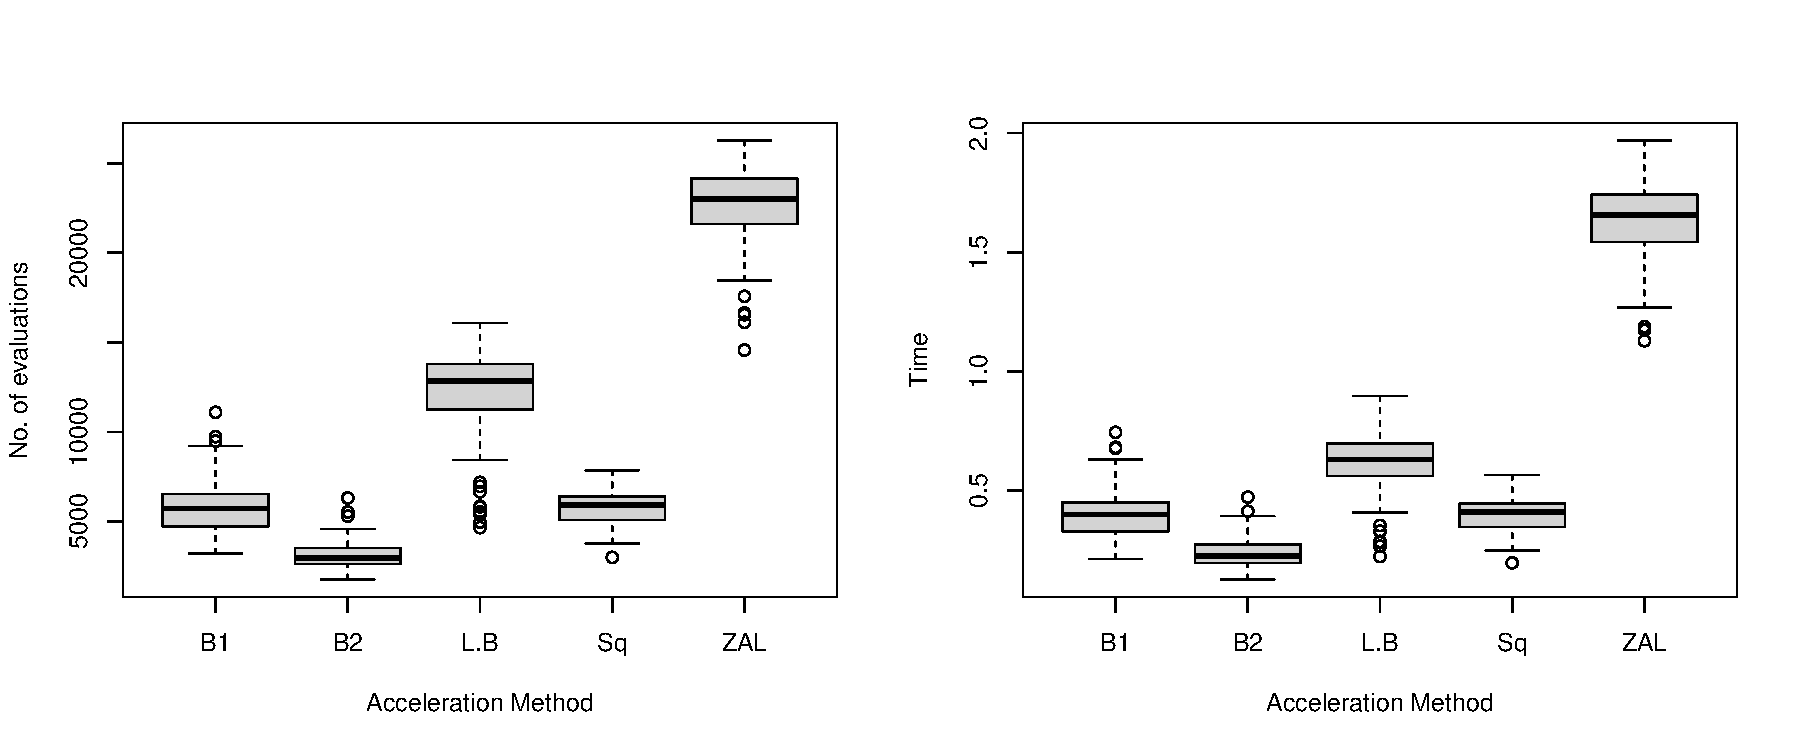
\includegraphics[width = \textwidth]{plots/quad-boxplot_sd1e3.pdf}
    \caption{Quadratic minimization: number of function  evaluations and runtime over $100$ random starting points. %Boxplots for number of iteration and time taken for 10 runs from randomly generated starting points. The starting values are generated randomly from a distribution centered at the true minima and with standard deviation of $1000$.}
    }
    \label{fig:quad_boxplot}
\end{figure}


\subsection{Truncated Beta Binomial} \label{ex:trunc.beta.binom}


We next consider a more difficult statistical optimization problem, turning to the cold incidence dataset by \cite{lidwell1951observations}.  These data have been modeled as a zero-truncated beta binomial model as the reported households have at least one cold incidence. %The households were classified as: (a) adults only; (b) adults and school children; (c) adults and infants; and (d) adults, school children, and infants. 
The data includes four different household types. We analyze the subset of data corresponding to all adult households here; further details on the data and results for other subsets of the data appear in Table~\ref{tab:beta_binom2} in the Appendix. Among adults, the number of households with $1, 2, 3, \text{ and }4$ cases are $15, 5, 2, \text{ and }2$ respectively.  %to present the results for the first category over here where 
%the number of household with $1, 2, 3, \text{and } 4$ cases are $15, 5, 2, 2$ respectively. 

Suppose $n$ is the total number of independent observations (households) and $x_i$ denotes the number of cold cases in the $i^{th}$ household. This can be modeled as a discrete probability model \citep{zhou2011quasi} with likelihood given by
\[
L(\theta | X) = \prod_{i=1}^{n}\dfrac{d(x_i| \theta)}{1-d(0|\theta)}\,.
\]
Here $d(x|\theta)$ is the probability density function for a beta binomial distribution with parameter vector $\theta$ and maximum count of $m=4$. Here $\theta = (\alpha, \pi)$ such that $\pi \in (0,1)$ and $\alpha >0$. We use MM algorithm to numerically maximize the likelihood function. The MM updates are given by 

\begin{align*}
    \alpha_{t+1} &= \dfrac{\sum_{j=0}^{m-1} (\dfrac{s_{1j}j \alpha_t}{\pi_t + j\alpha_t} + \dfrac{s_{2j}j \alpha_t}{1 - \pi_t + j\alpha_t})}{\sum_{j=0}^{m-1}\dfrac{r_j j }{1 + j \alpha_t}}\\
    \pi_{t+1} &= \dfrac{\sum_{j=0}^{m-1}\dfrac{s_{1j}\pi_t}{\pi_t + j\alpha_t}}{\sum_{j=0}^{m-1}(\dfrac{s_{1j \pi_t}}{\pi_t + j \alpha_t} + \dfrac{s_{2j}(1-\pi_t)}{1- \pi_t + j \alpha_t})}
\end{align*}
where $s_{1j}, \, s_{2j},\, r_j$ can be interpreted as pseudocounts, given by
\begin{align*}
    s_{1j} &= \sum_{i=1}^{n}1_{x_i \geq j+1}\\
    s_{2j} &= \sum_{i=1}^{n} \left[ 1_{x_i \leq m-j-1} + \dfrac{g(0|\pi_t, \alpha_t)}{1 - g(0 | \pi_t, \alpha_t)} \right]\\
    r_j &= \sum_{i=1}^{n}\left[ 1 +  \dfrac{g(0|\pi_t, \alpha_t)}{1 - g(0 | \pi_t, \alpha_t)} \right] 1_{t \geq j+1}\,.
\end{align*}



\begin{table}
\caption{\label{tab:beta_binom1} Truncated beta binomial: performance on Lidwell and Somerville
 data, from initial point $(\pi,\alpha) = (0.5, 1)$. } %the stopping criterion
%is $\epsilon = 10^{-7}$, and the number of parameters is two.}
\centering

\fbox{\begin{tabular}{ c c c c c} 
 \hline
  Algorithm & -ln L & $F$ Evals & Iterations & Time (in sec) \\ [0.5ex] 
 \hline
   MM & 25.2283 & 17898 & 17898 & 0.114 \\ 
    BQN ($q=1$) & 25.2287 & 26 & 14 & 0.001 \\
    BQN ($q=2$) & 25.2277 & 29 & 16 & 0.001\\
    L-BQN & 25.2288 & 73 & 37 & 0.002\\
    SqS1 & 25.2274 & 1797 & 1769 & 0.160\\
    SqS2 & 25.2277 & 36 & 19 & 0.004\\
    SqS3 & 25.2269 & 69 & 35 & 0.005\\
    ZAL & 25.2269 & 28 & 24 & 0.003\\[1ex]
  \hline
\end{tabular}}
\end{table}


\begin{figure}
     \centering
     \subfloat[MM]{ 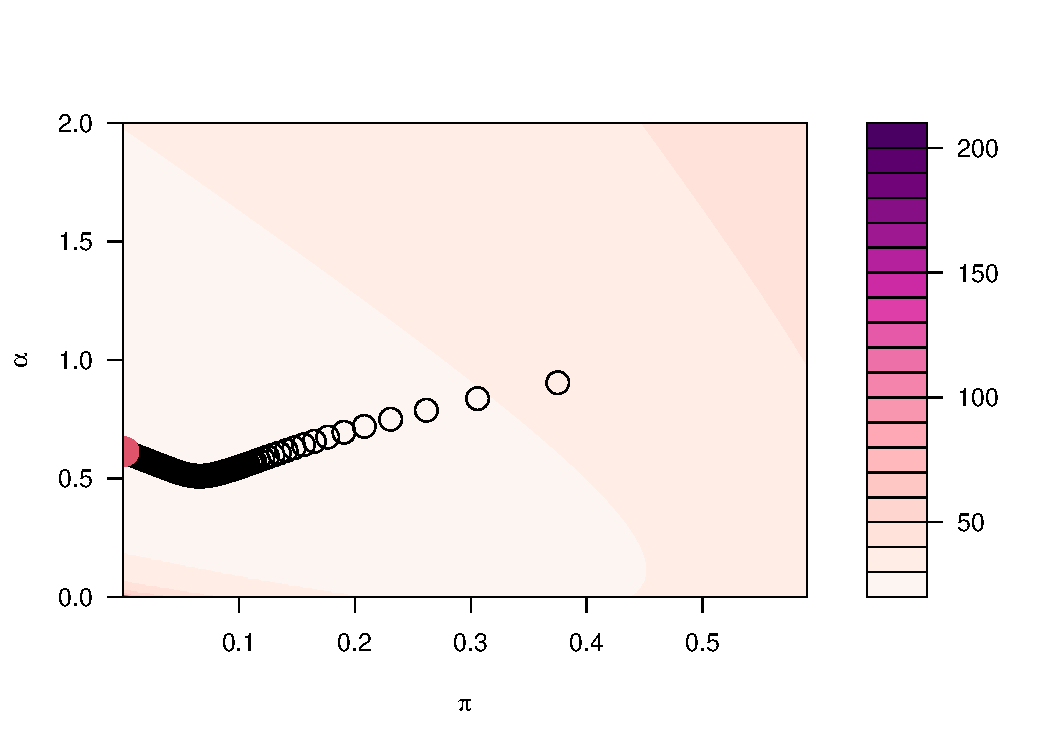
\includegraphics[width = .45\textwidth]{plots/beta-contour_MM.pdf}}
    \subfloat[BQN, $q=1$]{ 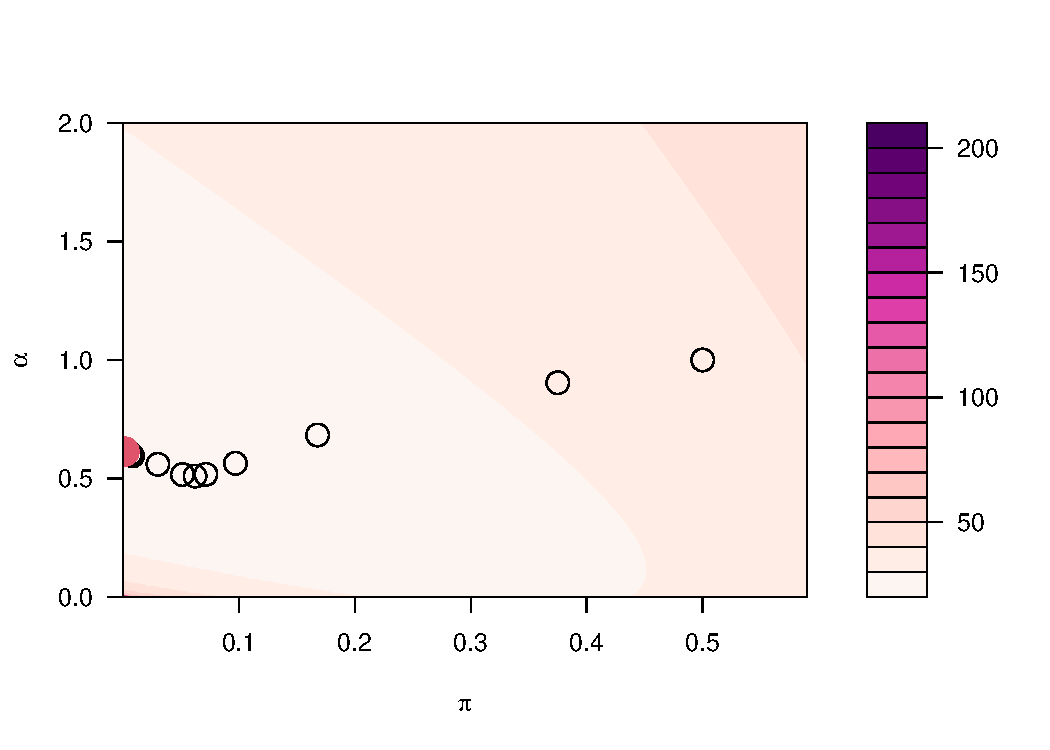
\includegraphics[width = .45\textwidth]{plots/beta-contour_BQN1.pdf}}\\
    \subfloat[BQN, $q=2$]{ 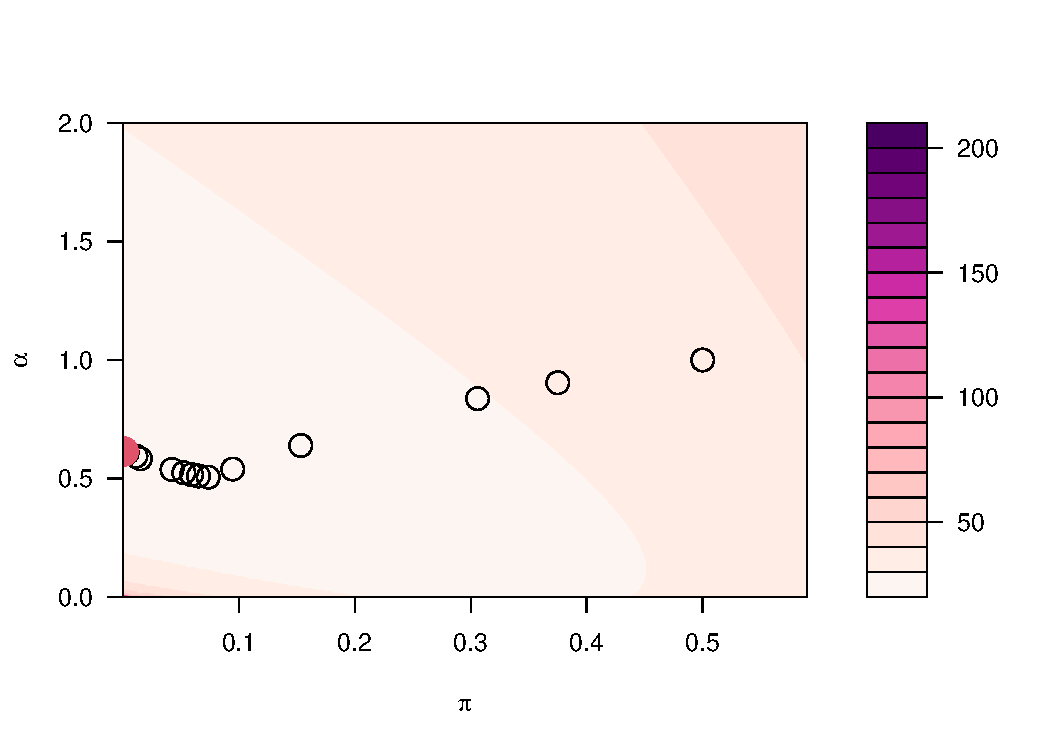
\includegraphics[width = .45\textwidth]{plots/beta-contour_BQN2.pdf}}
    \subfloat[L-BQN]{ 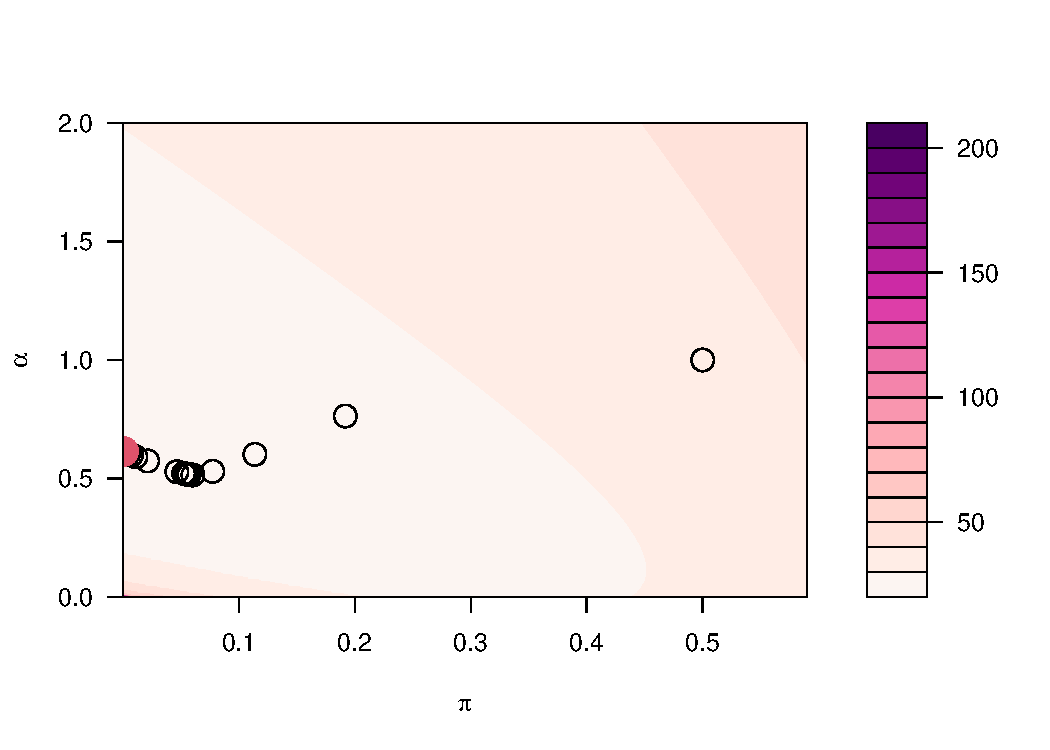
\includegraphics[width = .45\textwidth]{plots/beta-contour_LBQN.pdf}}\\
    \subfloat[SQUAREM-3]{ 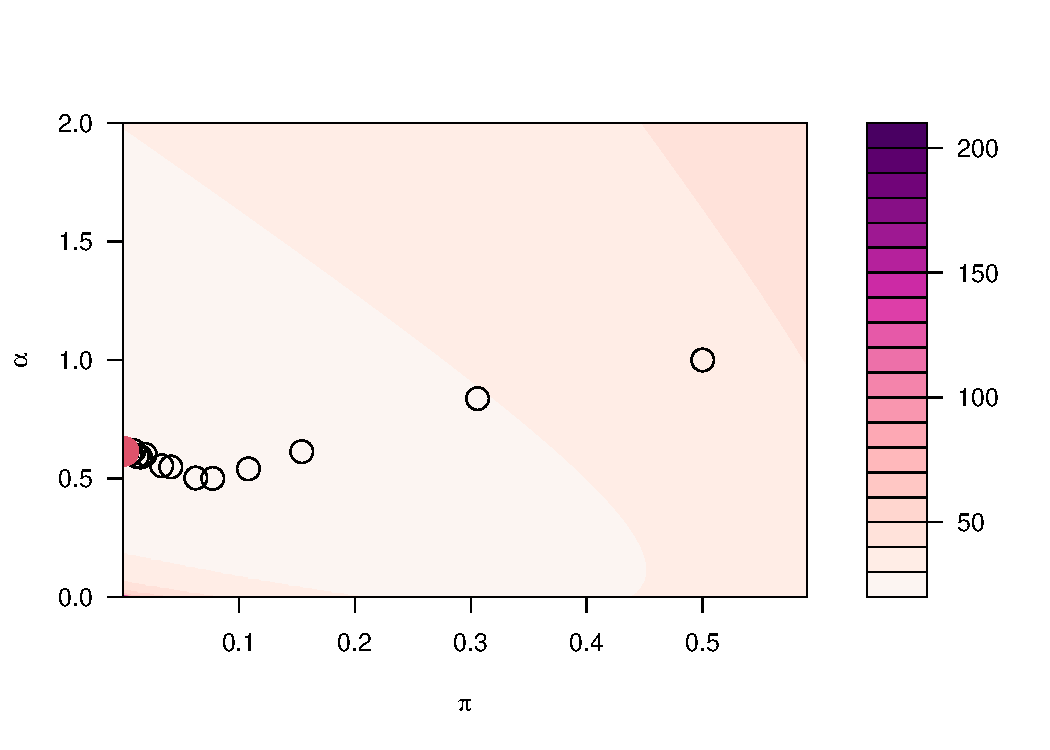
\includegraphics[width = .45\textwidth]{plots/beta-contour_SqS3.pdf}}
    \subfloat[ZAL, $q=1$]{ 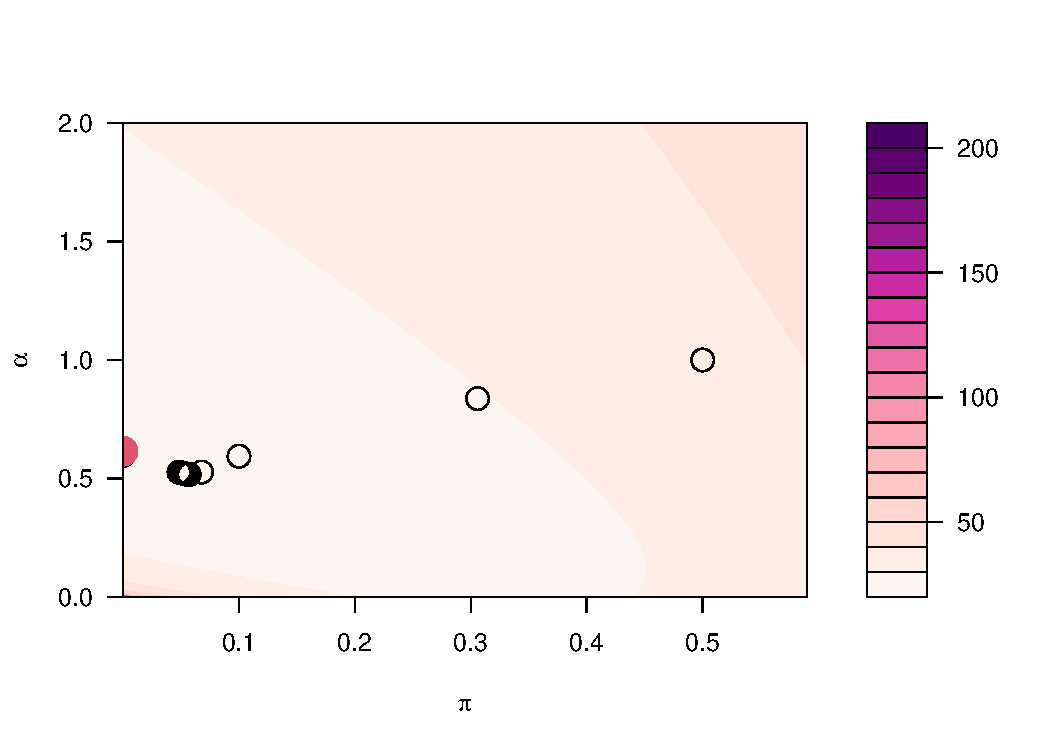
\includegraphics[width = .45\textwidth]{plots/beta-contour_ZAL.pdf}}
     
     \caption{Truncated beta binomial: ascent paths of peer methods on the Lidwell and Somerville household incidence data in a truncated beta binomial model, with  optimum marked in red.}%. The tolerance is $\epsilon = 10^{-7}$.}
    
     \label{fig:beta-contour}
 \end{figure}

Following \cite{zhou2011quasi}, each algorithm is  initializated at $(\pi, \alpha) = (0.5, 1)$. %and tolerance $\epsilon = 10^{-7}$, 
Table \ref{tab:beta_binom1} lists the negative log-likelihood values, number of MM evaluations (F evals), number of algorithm iterations, and runtime until convergence for each algorithm. %It can be observed that BQN with $q=2$ provides an improvement over $q=1$ case. F
Figure~\ref{fig:beta-contour} provides a closer look, showing the progress path of each algorithm on a contour plot of the objective. SQUAREM methods, though achieving significant acceleration, tend to exhibit slow tail behavior near the optimal value. In particular, SQUAREM-1 leads to orders of magnitude slower convergence than the others, while it outpaced other choices of steplength among variants of SQUAREM in the simple example; we again focus on visualizing the progress of the default SQUAREM-3. In all cases, our method converges in fewer iterations and requires fewer function evaluations than its competitors despite a naive implementation. From Figure~\ref{fig:beta-contour}, we can visualize the advantage of our extrapolation-based steps making steady progress, in contrast to the more congested updates near the optimum under existing methods. While the small problem dimension does not call for a limited-memory method, we see L-BQN also compares favorably despite its streamlined updates. % show that despite its matrix-based updates, it competes well with the scalar-based SQUAREM methods.



\subsection{Generalized eigenvalues} \label{ex:gen.eigen}


In this example, we consider a more complicated objective function that exhibits a zig-zag descent path under the na\"ive MM algorithm, rendering progress excruciatingly slow. For two $p \times p$ matrices $A$ and $B$, the generalized eigenvalue problem refers to finding a scalar $\lambda$ and a nontrivial vector $x$ such that $Ax = \lambda Bx$. We consider the case where $A$ is symmetric and $B$ is symmetric and positive definite, so that the generalized eigenvalues and eigenvectors are real %. For further details on different solutions to the problem in literature, refer to 
\citep{zhou2011quasi}. A simple alternative for finding the generalized eigenvalues iteratively is by optimizing the Rayleigh quotient 
\[
R(x) = \dfrac{x^T A x}{x^T B x} \qquad \qquad x \neq 0\,.
\]
The gradient of $R(x)$ is given by
\[
\nabla R(x) = \dfrac{2}{x^T B x}[Ax - R(x)Bx]\,.
\]

Therefore, a solution of $\nabla R(x)=0$ corresponds to a generalized eigenpair, wherein the maximum of $R(x)$ gives the maximum generalized eigenvalue and minimum gives the minimum generalized eigenvalue. %A candidate for optimizing $R(x)$ is  steepest ascent or descent; 
To optimize $R(x)$, we consider the line search method for steepest ascent proposed by \cite{hestenes1951solutions} as the base algorithm.


\begin{figure}
    \centering
    \subfloat[Smallest Eigenvalue]{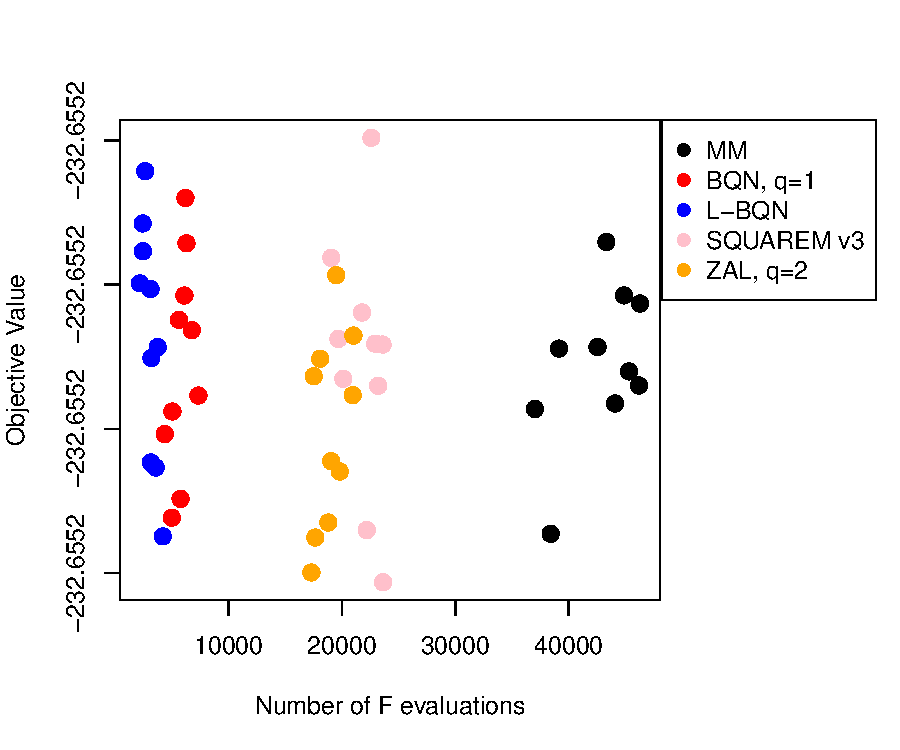
\includegraphics[width = .49\linewidth]{plots/eigen-objVSeval_descent.pdf}}
    \subfloat[Smallest Eigenvalue]{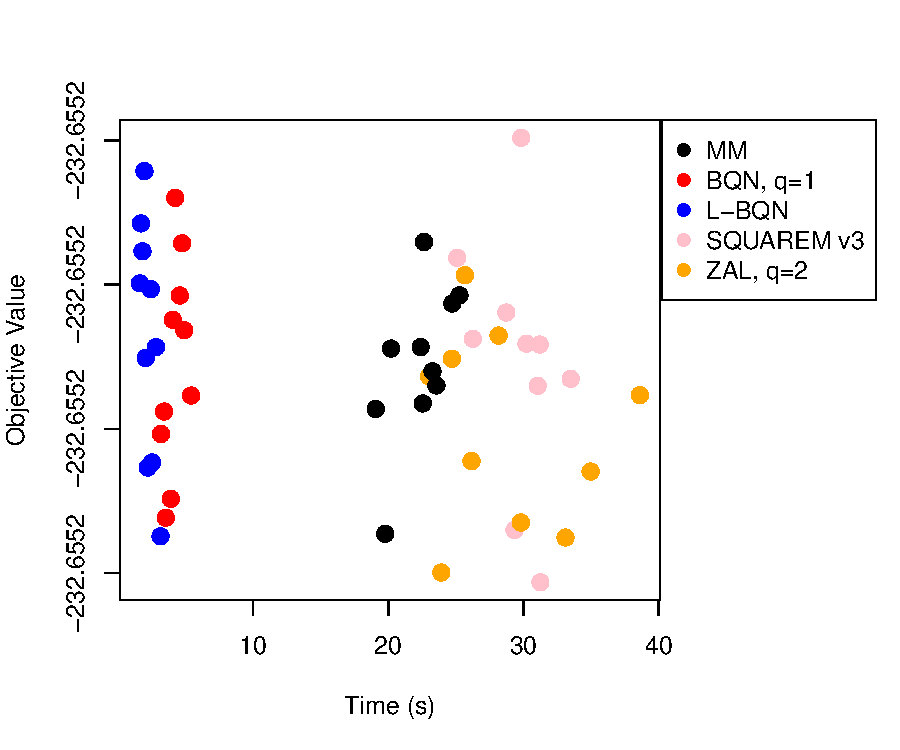
\includegraphics[width = .49\linewidth]{plots/eigen-objVStime_descent.pdf}}
    
    \subfloat[Largest Eigenvalue]{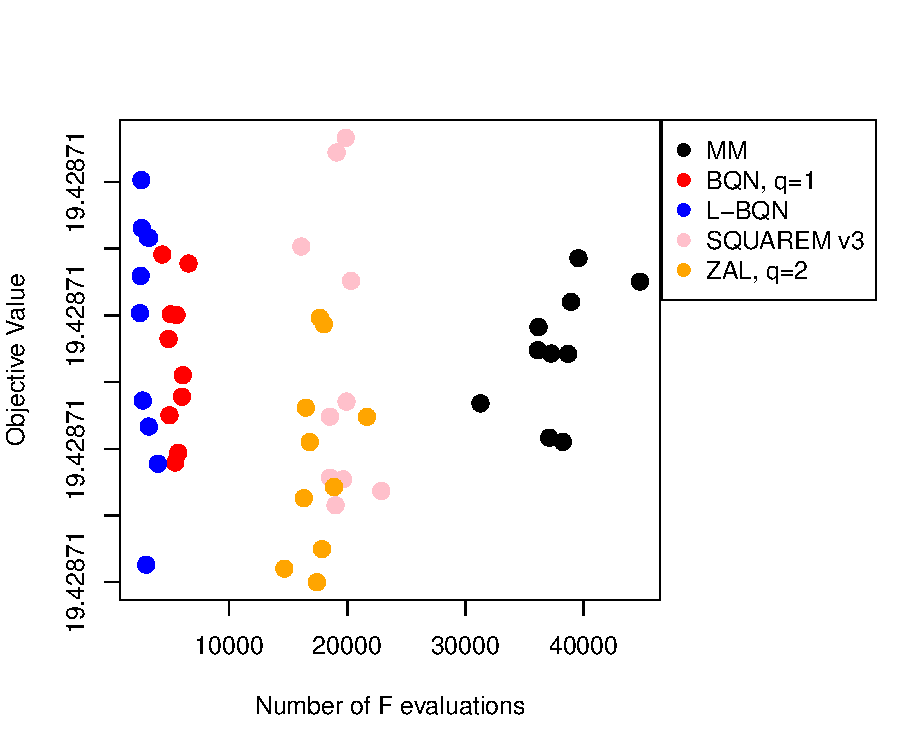
\includegraphics[width = .49\linewidth]{plots/eigen-objVSeval_ascent.pdf}}
    \subfloat[Largest Eigenvalue]{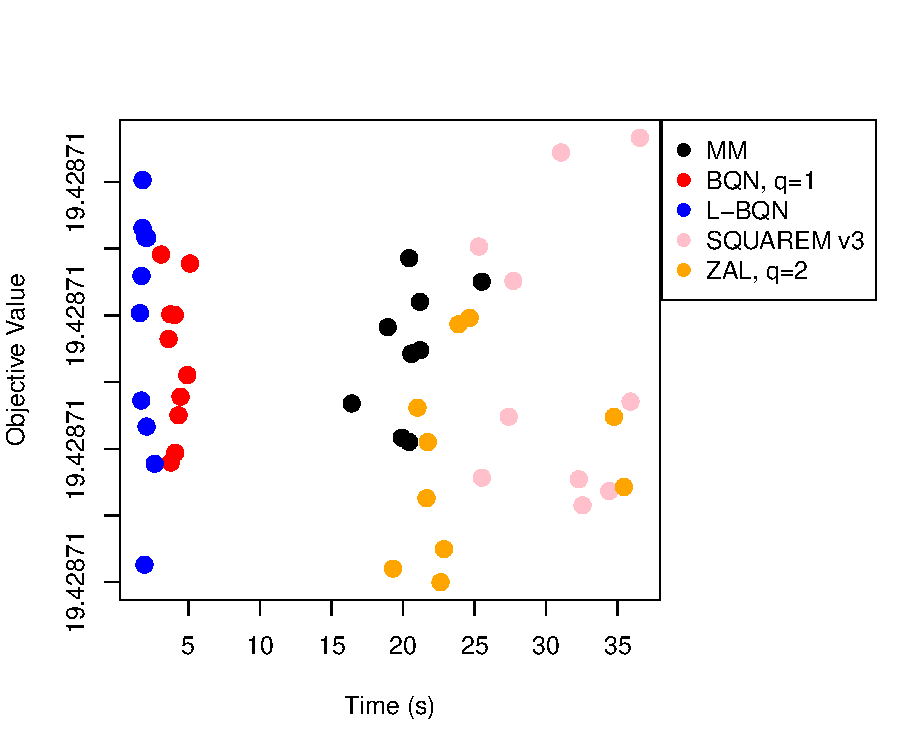
\includegraphics[width = .49\linewidth]{plots/eigen-objVStime_ascent.pdf}}
    
    \caption{Generalized eigenvalues: objectives at convergence over $10$ restarts vs the time and number of F evaluations. }% Convergence value of objective vs no. of function evaluations scatter plot for $N=10$ replications. The stopping criteria is $\epsilon  = 10^{-7}$. Lower objective is better. }
    \label{fig:eigen-sp}
\end{figure}

\begin{table}
\caption{\label{tab:gen_eigen}
Generalized eigenvalues: number of $F(x)$ evaluations, runtime, and eigenvalues at convergence.}% for $p=100$. A and B are randomly generated. The stopping criterion is $\epsilon = 10^{-7}$. The starting vector is randomly chosen.}

\centering
\fbox{%
\begin{tabular}{c | c c c | c c c} 
 \hline
  & \multicolumn{3}{|c|}{Smallest Eigenvalue} & \multicolumn{3}{c}{Largest Eigenvalue} \\ [0.5ex] 
Algorithm & Time (in sec) & $F$ Evals & Eigenvalue & Time (in sec) & $F$ Evals  & Eigenvalue\\ [0.5ex]
 \hline
MM  & 10.104 & 42552 & -232.6552 & 8.539 & 38262 & 19.4287\\ 
BQN, $q=1$ & 2.046 & 6682 & -232.6552 & 1.854 & 5766 & 19.4287\\
L-BQN & 1.203 & 4046 & -232.6552 & 0.664 & 2399 & 19.4287\\
SqS1 & 11.850  & 21777 & -232.6552 & 11.397 & 19642 & 19.4287 \\
SqS2 & 12.391 & 21777 & -232.6552 & 11.003 & 19642 & 19.4287 \\
SqS3 & 12.525 & 21777 & -232.6552 & 11.021 & 19642 & 19.4287\\
ZAL & 9.979 & 17920 & -232.6552 & 9.665 & 17415 & 19.4287\\ [1ex] 
 \hline
\end{tabular}}
\end{table}


Due to the zigzag nature of steepest ascent on this problem, \cite{zhou2011quasi} found na\"ive acceleration to perform poorly. Utilizing this side information, they considered instead the $s$-fold functional composition of the base algorithm for $s$ even as the underlying map, improving performance. We refrain from using the same heuristic in order to illustrate the  off-the-shelf applicability of our method. %We present the results for $p=100$ dimensional problem with tolerance $\epsilon = 10^{-7}$. 
We consider a simulation study with symmetric matrices $A$ and $B$ randomly generated with $p=100$ dimensions, and run $10$ random initializations of each method from matched initial points.  % for ten independent runs, all initialized at matching randomly generated starting points for each algorithm.

 Figure~\ref{fig:eigen-sp} displays objective values at convergence, and Table \ref{tab:gen_eigen} details the results. It can be seen that without the $s$-fold functional composition, both SQUAREM and ZAL fails to accelerate meaningfully here. On the other hand, the curvature information is crucial toward informing a good search direction in such cases, and our formulation successfully leverages this information. % this type of zig-zag objective to make the right choice of search direction. 
 This information is largely ignored in the scalar based methods SQUAREM, while ZAL attempts to make use of curvature information under an assumption that it is close to the stationary point. 

 
 %While the fallback mechanism employed by ZAL scheme ensures that the number of $F$ function evaluations are less than or equal to that of vanilla MM implementation, surely ZAL takes more time since a wrong search direction is suggested on every iteration. Again the partial monotonic nature of SQUAREM ensures a lower number of $F$ evaluations than plain MM algorithm, but it cannot be inferred as acceleration due to higher time required until convergence. 


 \subsection{Multivariate t-distribution} \label{ex:multi.t.distr}
 
 Our last example turns to estimation under a multivariate $t$-distribution, a robust alternative to  multivariate normal modeling when the errors involve heavy tails \citep{lange1989robust}.  %We compare the performance of BQN acceleration scheme to other quasi-Newton methods discussed before in a high-dimensional case. 
 \cite{varadhan2008simple} considered this example to compare SQUAREM to standard EM as well as PX-EM, an efficient data augmentation method  \citep{meng1997algorithm}. %The reason why their data augmentation method fits into parameter expansion paradigm can be seen in the discussion section of \cite{varadhan2008simple}. 
 %However, we will not implement the PX-EM acceleration because it is problem specific and cannot be applied in a generalized setting. \\
 
 Suppose we have $p$-dimensional data $Y = (y_1, ..., y_N)$ that we wish to fit to a multivariate $t$-distribution with unknown degrees of freedom $\nu$. The density is given by 
 \[
 f(y| \mu, \Sigma) \propto | \Sigma |^{-1/2} \left(\nu + (y - \mu)^T \Sigma^{-1} (y - \mu)\right)^{(\nu + p)/2},
 \]
and so the data likelihood is givein by $\prod_{i=1}^{N}f(y_i | \mu, \Sigma)$. There is no closed form solution to find $(\mu, \Sigma)$ which maximize the likelihood, but we can make progress by augmenting the missing data with latent variables. That is, we obtain the complete data $\{(y_i, q_i); i = 1, ..., N\}$ where q are IID from $\chi^2_\nu / \nu$;  the maximum likelihood estimator (MLE) now follows from weighted least squares. In an EM algorithm, the E-step finds the expected complete data log-likelihood conditional on parameters from the previous iteration $k$. %, conditionally on $Y$ and $(\mu_k, \Sigma_k)$ from the previous iteration $k$.  
Conditional on $Y$ and $(\mu_k, \Sigma_k)$, the latent variables are distributed as $q_i \sim \chi^2_{\nu +p}/(\nu + d_i^{(k)})$, where $d_i^{(k)} = (y_i - \mu_k)^T \Sigma_k^{-1} (y_i - \mu_k); i= 1,..., N$. As the complete-data log-likelihood is linear in $q_i$, the E-step amounts to defining
 \[
 w_i = E[q_i | y_i, \mu_k, \Sigma_k] = (\nu + p)/(\nu + d_i^{(k)}); \qquad i = 1, ..., N\,.
 \]
 The M-step then yields:
 \begin{align*}
     \mu_{k+1} &=\sum_{i}w_i y_i \bigg / \sum_{i}w_i\,, \qquad \Sigma_{k+1} \,=\, \dfrac{1}{N} w_i (y_i - \mu)(y_i - \mu)^T\,.
 \end{align*}
 
\begin{table}
    \caption{\label{tab:t-dist}%Multivariate t-distribution. 
    Multivariate t-distribution: maximum likelihood estimation of a 25-dimensional multivariate t-distribution. } 

    \centering
\fbox{\begin{tabular}{c c c c} 
 \hline
 Algorithm & $F$ Evals & Time (in sec)  & $-\ln L$ \\ [0.5ex] 
 \hline
 EM & 744 & 1.086 & 8608.993\\ 
 PX-EM & 38 &  0.063 & 8608.993\\
 BQN, $q=1$ & 112 & 0.215 & 8608.993\\
 BQN, $q=2$ & 223 & 0.457 &  8608.993\\
 L-BQN & 89 & 0.114 & 8608.993\\
 SqS1 & 64 & 0.156 & 8608.993\\
 SqS2 & 65 & 0.148 & 8608.993\\
 SqS3 & 63 & 0.155 & 8608.993\\
 ZAL, $q = 2$ &  383 & 1.383 &  8608.993\\
 [1ex] 
 \hline
\end{tabular}
}
\end{table}

 The PX-EM method of \cite{meng1997algorithm} differs only in the $\Sigma$ update, replacing the denominator N by $\sum_{i}w_i$. We randomly generate synthetic data with $\nu = 1$ (a multivariate Cauchy distribution) and parameters $\mu = 0$, $\Sigma = V$, where $V$ is a symmetric randomly generated matrix with dimension $p = 25$, which corresponds to $350$ parameters (25 for $\mu$ and 325 for $\Sigma$). % and $\epsilon = 10^{-7}$. 
  We report results obtained from following the initial values suggested by \cite{meng1997algorithm}:
 
 \begin{equation*}
     \mu_0 =  \dfrac{1}{N}\sum_{i=1}^{N}y_i, \qquad
     \Sigma_0 = \dfrac{1}{N}\sum_{i=1}^{N}(y_i - \overline{y})(y_i - \overline{y})^T\,.
 \end{equation*}
 
 Table~\ref{tab:t-dist} displays runtime, number of $F$ evaluations (F evals), and negative log likelihood of all acceleration schemes at convergence. Our method achieves significant acceleration compared to the standard EM algorithm and performs on par with SQUAREM while outpacing ZAL. Here ZAL fails to provide meaningful acceleration under its implementation in \texttt{turboEM}---we observe it frequently proposes an update such that $\Sigma_k$ is not positive-definite. In these cases, the algorithm reverts to the default MM update, adding additional computational effort, though the implementation in \cite{zhou2011quasi} achieves more success. Though performance is always quite dependent on implementations, we echo the overall theme in the findings of \cite{varadhan2008simple,zhou2011quasi} that  model-specific augmentation under PX-EM performs remarkably well, outpacing all of the more general methods. This example illustrates that despite the robust performance of our proposed method across settings, it is worthwhile to exploit problem-specific structure as does PX-EM whenever possible.


% \subsection{Examples} \label{subsec:L-BFGSex}


% The prime motivation for the following experiments is to compare the performance of limited memory BFGS, standard BFGS, SQUAREM and ZAL for high dimensional cases. The limited memory method is implemented by storing a certain $m$ number of n-dimensional vector pairs $(u_i, v_i)$ instead of storing the entire $n \times n$ Hessian matrix $H_i$. For our experiments, we will use $m=10$. We stop at iteration $t$ whenever $\|F(x_t) - x_t\|^2 \leq \epsilon$ where $\epsilon = 10^{-7}$. Two examples from section \ref{subsec:BFGSex} have been modified to a high dimensional case and compared to other methods. These are a) Multivariate t-distribution and b) generalized Eigenvalues examples.

% \subsubsection{Multivariate t-distribution}

% Like example \ref{ex:multi.t.distr}, we try to fit a Cauchy model ($\nu = 1$) to data generated from multivariate t-distribution. There is no closed form MLE solution but using the data augmentation technique, one can find the MLE using weighted least squares method. We will accelerate the EM algorithm described by \cite{varadhan2008simple} for a $p = 50$ which accounts for 1325 parameters (50 for $\mu$ and 1275 for the symmetric matrix $\Sigma$). The data is generated from using $\mu = \textbf{0}$ and a randomly generated covariance matrix.\\
% \\
% It can been in Table \ref{tab:t-dist2} that L-BFGS performs way better than BFGS based quasi Newton method with respect to running time. This can be attributed to high time and memory requirements associated with BFGS method in storing and performing matrix multiplication for $1325 \times 1325$ Hessian matrices.
% \begin{table}[h!]
% \centering
% \begin{tabular}{c c c c c} 
%  \hline
%  Algorithm & Fevals & Levals & Time & Likelihood\\ [0.5ex] 
%  \hline
%  EM & 1007 & 1007 & 3.7911  & -19322.47\\ 
%  PX-EM & 50 & 50 & 0.2263 & -19322.47 \\
%  ZAL & 1046 & 1046 & 7.3111 & -19322.47 \\
%  SqS1 & 114 & 46 & 0.6382 &  -19322.47 \\
%  SqS2 & 102 & 44 & 0.5794 & -19322.47 \\
%  SqS3 & 87 & 37 & 0.4627 & -19322.47\\
%  BFGS & 141 & 141 &  110.892 & -19322.47\\
%  L-BFGS & 114 & 46 & 0.5625 & -19322.47 \\
%  JJ-QN1 & 66 & 0 & 1.6766 & -19322.47 \\[1ex] 
%  \hline
% \end{tabular}
% \caption{Parameter estimation of a 1325-dimensional multivariate t-distribution, with 1 degree of freedom with $\mu = 0$, and a randomly generated covariance matrix.}
% \label{tab:t-dist2}
% \end{table}
\section{Conclusion}

This article presents a novel quasi-Newton acceleration of MM algorithms that extends recent ideas, but lends them new intuition as well as theoretical guarantees. % that does not require the original quantity been optimized. Furthermore, t
The method  retains gradient information across all components, which is often ignored in other \textit{pure} MM accelerators. % (see \cite{jamshidian1997acceleration}). 
A key advantage of MM algorithms is their transfer of difficulty away from the original objective function, obtained by the construction of surrogates. While the \textit{hybrid} quasi-Newton MM accelerators \citep{lange1995quasi, heiser1995convergent, lange2000optimization} are rigorously analyzed in the literature, they lose this appeal in part by requiring information from the original objective through their iterates. Our approach seeks to embody the best of both worlds,  retaining the simplicity of pure accelerators without restrictive assumptions, maintaining computational tractability so that it is amenable for large and high-dimensional problems, and taking advantage of richer curvature information that yields classical convergence guarantees which may not hold for its peer methods.

The limited-memory version of our method performs well on our representative, but not exhaustive, set of examples. As this  shows promise toward high-dimensional problems, a fruitful line of research may seek to study the convergence properties of L-BQN explicitly, building on prior analyses on  convergence of limited memory BFGS method \citep{liu1989limited}. Exploring optimal step size selection presents another open direction \citep{nocedal2006numerical}. Despite deriving from a different perspective, it is satisfying that the steplength for our inverse Jacobian update in Eq.\eqref{eq:BFGS_update} reveals that used for the first version of STEM as a special case \cite{varadhan2008simple}. Nonetheless, exploring the practical and theoretical merits of alternatives may reap further advantages. % \cite{nocedal2006numerical}. %% A further line of thought is to explore the other two formulations for steplength and compare their properties. See \cite{nocedal2006numerical} for discussion on steplengths. 

%In our discussion, we have focused on the \textit{pure} category of quasi-Newton methods for MM acceleration. However, when evaluating the objective or its derivatives is straightforward, there are various quasi-Newton acceleration methods with promising results. A valuable line of research would be to compare the two classes by studying their theoretical and experimental properties.

\bibliographystyle{rss}
\bibliography{example}

\section{Appendix} \label{sec:appendix}

\subsection{Proof of Theorem~\ref{th:convergence}}
Let $\mathbb{R}^{p\times p}$ denote linear space of real matrices of order $p \times p$. Recall that $\|A\|_M := \|MAM\|_F$ is a matrix norm of matrix $A$ for any matrix $M$, $\|\cdot\|_F$ is the Frobenius norm, and $\|\cdot\|$ denotes a vector norm or its induced operator norm. 
\begin{proof}[]
The proof argues that if $\bx_0 \in D$, then $\bx_1$ also lies in D using the inequality in Eq.\eqref{eq:jacobian_error}. Additionally, it is shown that the distance of $\bx_1$ from $\bx^\ast$ is less than or equal to some $r$th fraction of the distance of $\bx_0$ from $\bx^\ast$. By induction, we prove that $\bx_i \in D$ for all $i \geq 1$, and eventually converge to $\bx^\ast$ with $r$ rate of convergence.

To this end, we upper bound the norm of the Jacobian and inverse Jacobian matrices at $\bx^\ast$ as $ \|dG(\bx^\ast)\| \leq \sigma \text{ and } \|dG(\bx^\ast)^{-1}\| \leq \gamma$. For any $r \in (0,1)$, we can choose $\epsilon(r) = \epsilon \text{ and } \delta(r) = \delta$ such that
\begin{align}
    [2\alpha_1\delta + \alpha_2] \dfrac{\epsilon^d}{1 - r^d} &\leq \delta \label{eq:epsilon_delta1}\\ 
    2\sigma \delta \eta + (\gamma + 2\eta \delta)K \epsilon^d &\leq r \label{eq:epsilon_delta2} \,.
\end{align}
If necessary, we may further restrict $\epsilon$ and $\delta$ such that $(\bx,H) \in N$ whenever $\|\bx - \bx^\ast\| < \epsilon$ and $\|H -dG(\bx^\ast)^{-1}\|_M~<~2\delta$. Now suppose $\|\bx_0 - \bx^\ast\| < \epsilon \text{ and } \|H_0 - dG(\bx^\ast)^{-1}\|_M < \delta$. Then  $\|H_0 - dG(\bx^\ast)^{-1}\| < \eta \delta < 2\eta \delta$ by the equivalence of norms in finite-dimensional vector spaces. From Eq.\eqref{eq:epsilon_delta2}, $2 \sigma \delta \eta \leq 2r$, and therefore the Banach lemma gives,
\[
\|H_0^{-1}\| \leq \dfrac{\sigma}{1-r}\,.
\]
Now, we will show that if $\bx_0 \in D$, then $\bx_1$ also lies in $D$. For this purpose, we add and subtract $H_0 dG(\bx^\ast)(\bx_0 - \bx^\ast)$ and add the null term $H_0G(\bx^\ast)$ to the known update formulation for $\bx_1$ giving
\begin{align*}
    \bx_1 - \bx^\ast &= \bx_0 - H_0G(\bx_0) - \bx^\ast \\
    &= -H_0\left[G(\bx_0) - G(\bx^\ast) - dG(\bx^\ast)(\bx_0 - \bx^\ast)\right] + \left[I_p - H_0dG(\bx^\ast)\right](\bx_0 - \bx^\ast)\,.
\end{align*}
Using the fact that $\|I_p - H_0dG(\bx^\ast)\| = \|dG(\bx^\ast)(H_0 - dG(\bx^\ast)^{-1})\| \leq \|dG(\bx^\ast)\|\|H_0 - dG(\bx^\ast)^{-1}\| \leq \sigma (2  \delta \eta)$ and Inequality \eqref{eq:ineq1},
\begin{align*}
    \|\bx_1 - \bx^\ast\| &\leq \|H_0\|K\epsilon^d\|\bx_0 - \bx^\ast\| + 2\sigma \delta \eta \|\bx_0 - \bx^\ast\|
    &= \left[\|H_0\|K \epsilon^d + 2 \sigma \epsilon \delta \eta\right]\|\bx_0 - \bx^\ast\|\,.
\end{align*}
But $\|H_0\| \leq \|H_0 - dG(\bx^\ast)^{-1}\| + \|dG(\bx^\ast)^{-1}\| \leq 2 \eta \delta + \gamma$. Therefore,
\[
\|\bx_1 - \bx^\ast\| \leq [(2 \eta \delta + \gamma)K \epsilon^d + 2 \sigma \epsilon \delta \eta]\|\bx_0 - \bx^\ast\| \leq r\|\bx_0 - \bx^\ast\|
\]
using the inequality in Eq.\eqref{eq:epsilon_delta2}, and hence $\bx_1 \in D$. The rest of the proof proceeds by induction. Assume that $\|H_k - dG(\bx^\ast)^{-1}\|_M < 2\delta$,  which implies  $ H_k \in N_2$ and $\|\bx_{k+1} - \bx^\ast\| \leq r\|\bx_k - \bx^\ast\|$ for $k = 0, 1, \dots, m-1$. Now since $\bx_k \in N_1 \subseteq S$, we have $\|F(\bx_k) - \bx^\ast\|^d \leq \tau^d \|\bx_k - \bx^\ast\|^d$ by the local convergence of the MM algorithm in $S$. It follows from the inequality in Eq.\eqref{eq:jacobian_error} that
\begin{align*}
    \|H_{k+1} - dG(\bx^\ast)^{-1}\|_M - \|H_k - dG(\bx^\ast)^{-1}\|_M &\leq \alpha_1\|\bx_k - \bx^\ast\|^d\|H_k - dG(\bx^\ast)^{-1}\|_M + \alpha_2 \|\bx_k - \bx^\ast\|^d \\
    &\leq \alpha_1 (r^{kd}\epsilon^d)(2\delta) + \alpha_2 r^{kd}\epsilon^d\,.
\end{align*}
Therefore, from the inequality in Eq.\eqref{eq:epsilon_delta1}, we have
\[
\|H_m - dG(\bx^\ast)^{-1}\|_M \leq \|H_0 - dG(\bx^\ast)^{-1}\|_M + (2 \alpha_1 \delta + \alpha_2)\dfrac{\epsilon^d}{1 - r^d} \leq 2\delta\,.
\]
In this way, the induction step is completed by following the same proof as the case for $m=1$. In particular, since $\|H_m - dG(\bx^\ast)^{-1}\| \leq 2\eta \delta$, the Banach lemma implies that
\[
\|H_m^{-1}\| \leq \dfrac{\sigma}{1-r}\,.
\]

\end{proof}

\subsection{Proof of Theorem 2}

In order to show that our algorithm satisfies \eqref{eq:jacobian_error} for meeting the conditions of Theorem~\ref{th:convergence}, we write \eqref{eq:BFGS_update} as
\begin{equation} \label{eq:MEM}
    \bar{E} = E\left[I_p - \dfrac{M^{-1}\bv(M\bv)^T}{\|\bv\|^2}\right] + \dfrac{M(\bu - dG(\bx^\ast)^{-1}v)(M\bv)^T}{\|\bv\|^2},
\end{equation}
where $\bar{E} = M(\bar{H} - dG(\bx^\ast)^{-1})M \text{ and } E = M(H - dG(\bx^\ast)^{-1})M$. Eq.\eqref{eq:MEM} will allow us to derive the relationship between $\|H-dG(\bx^\ast)^{-1}\|_M$ and $\|\bar{H}-dG(\bx^\ast)^{-1}\|_M$ satisfying the inequality in \eqref{eq:jacobian_error}. For this purpose, we present the following technical lemma with four important inequalities satisfied by our algorithm. Since our update formulation falls in the classical line of thought, we inherit the following properties directly from the analysis presented by \cite{broyden1973local}, so the proofs have been omitted. Nonetheless, the results have been included for the sake of completion for Theorem~\ref{th:qnm_convergence}.
\begin{lemma} \label{lemma:MEM}

Let $M \in \mathbb{R}^{p\times p}$ be a non-singular symmetric matrix such that
\begin{equation} \label{eq:lemma2_condition}
    \|M\bc - M^{-1}\bd\| \leq \beta \|M^{-1}\bd\|
\end{equation}
for some $\beta \in [0, 1/3]$ and vectors $\bc$ and $\bd$ in $\mathbb{R}^p$ with $\bd \neq \mathbf{0}$. Then using $E$ and $\bar{E}$ as defined earlier,
\begin{enumerate}
    \item $(1 - \beta)\|M^{-1}\bd\|^2 \leq \bc^T\bd \leq (1 + \beta) \|M^{-1}\bd\|^2$\,.
    \item $E\left[I - \dfrac{(M^{-1}\bd(M^{-1}\bd)^T}{\bc^T\bd}\right] \leq \sqrt{1 - \alpha \theta^2} \|E\|_F$\,.
    \item $\left\|E \left[I - \dfrac{M^{-1}\bd (M\bc)^T}{\bc^T\bd}\right]\right\|_F \leq \left[ \sqrt{1 - \alpha \theta^2} + (1-\beta)^{-1} \dfrac{\|M\bc - M^{-1}\bd\|}{\|M^{-1}\bd\|} \right]\|E\|_F $\,, \\
    where
    \[
    \alpha = \dfrac{1 - 2\beta}{1  - \beta^2} \in [3/8, 1]
    \]
    and 
    \[
    \theta  = \dfrac{\|EM^{-1}\bd\|}{\|E\|_F\|M^{-1}\bd\|} \in [0,1]\,.
    \]
    Moreover, for any $\ba \in \mathbb{R}^p$,
    
    \item $\left\| \dfrac{(\ba - dG(\bx^\ast)^{-1}\bd)(M\bc)^T}{\bc^T\bd} \right\|_F \leq 2\dfrac{\|\ba - dG(\bx^\ast)^{-1}\bd\|}{\|M^{-1}\bd\|}$\,.
\end{enumerate}
\end{lemma}
In the following proof, we will use results from the above lemma with $\bc = \bv$, $\bd= \bv$, and result $(d)$ particularly for $\ba = \bu$. We are now ready to show that the conditions of Theorem~\ref{th:convergence} are satisfied by our update formula. This allows us to construct the exact neighborhood for each $r \in (0,1)$ wherein our algorithm converges to the stationary point with rate $r$.

\begin{proof}[Theorem~\ref{th:qnm_convergence}]
Firstly, we construct the neighborhoods $N_1$ and $N_2$ wherein our the updates in \eqref{eq:QN_update} and \eqref{eq:BFGS_update} are well-defined. Define $N_2 = \{H \in \mathbb{R}^{p\times p}: \|dG(\bx^\ast)\|\|H - dG(\bx^\ast)^{-1}\| < 1/2\}$ such that each $H \in N_2$ is non-singular, and there exists a constant $\nu > 0$ such that $\|H\| \leq \nu$ for all $H \in N_2$. Using Lemma~\ref{lemma:lipchitz}, we we also choose $\epsilon \text{ and } \rho$ such that $\max\{\|\bar{\bx} - \bx^\ast\|^d, \|\bx-\bx^\ast\|^d\} \leq \epsilon$ implies that \eqref{eq:ineq2} holds. In particular, if $\|\bx - \bx^\ast\| \leq \epsilon$ and $H \in N_2$, then $\bx \in D$ and 
\[
(1/\rho)\|\bx - \bx^\ast\| \leq \|G(\bx)\| \leq \rho \|\bx - \bx^\ast\|\,.
\]
As a consequence of applying the inequality above on Eq.\eqref{eq:QN_update}, we have
\[
\|\bs\| \leq \|H\|\|G(\bx)\| \leq \rho \|H\| \|\bx - \bx^\ast\| \leq \rho \nu \|\bx- \bx^\ast\|\,.
\]
Now define $N_1$ as the set of all $\bx\in \mathbb{R}^p$ such that 
\[
\|\bx - \bx^\ast\| < \min\{\epsilon/2, \epsilon/(2\rho), \epsilon/(2\rho \nu)\}
\]
where $\rho \epsilon < (3\mu_2)^{-1/d}$. Now if $\bx \in N_1$ then
\begin{align} \label{eq:ineq4}
    \|\bs\| &\leq \rho \nu \|\bx-\bx^\ast\| \leq \epsilon/2 \qquad \text{ and } \qquad
    \|F(\bx) - \bx\| \leq \rho \|\bx - \bx^\ast\| \leq \epsilon/2\,.
\end{align}
If $N = ((N_1 \cap S) \times N_2) \cap N^\prime$ and $(\bx, H) \in N$, then $\bx, \bar{\bx}, \text{ and } F(\bx)$ lie in $D$ because using \eqref{eq:ineq4}
\[
\|\bar{\bx} - \bx^\ast\| \leq \|\bs\| + \|\bx - \bx^\ast\| \leq \epsilon \quad \text{and} \quad \|\bar{F(\bx)} - \bx^\ast\| \leq \|F(\bx) - \bx\| + \|\bx - \bx^\ast\| \leq \epsilon\,.
\]
Hence Inequality \eqref{eq:ineq2} shows that
\begin{subequations} 
\begin{align}
    \left(\dfrac{1}{\rho}\right)\|\bs\| &\leq \|\by\| \leq \rho \|\bs\|\,,\\
    \left(\dfrac{1}{\rho}\right)\|\bu\| &\leq \|\bv\| \leq \rho \|\bu\|\,, \label{eq:uv_ineq}
\end{align}
\end{subequations}

and in particular
\begin{subequations}
\begin{align}
    \mu_2 \|\by\|^d &\leq \mu_2 (\rho \epsilon)^d \leq 1/3\\
    \mu_2 \|\bv\|^d &\leq \mu_2 (\rho \epsilon)^d \leq 1/3\,. \label{eq:beta_value}
\end{align}
\end{subequations}
Thus $\by=0$ if and only if $\bs=0$, which happens if and only if $\bx=\bx^\ast$. This shows that the update function in Eq.\eqref{eq:QN_update} and \eqref{eq:BFGS_update} is well-defined for all $(\bx,H) \in N$. We now show that the update functions satisfy the conditions of Theorem \ref{th:convergence}. Since \eqref{eq:ineq3} and \eqref{eq:beta_value} imply that \eqref{eq:lemma2_condition} hold with $\beta = 1/3$, it follows from \eqref{eq:ineq3} and parts $(c)$, $(d)$ of Lemma \ref{lemma:MEM} applied on \eqref{eq:MEM} that
\begin{align*}
    \|\bar{H} - dG(\bx^\ast)^{-1}\|_M &\leq \left[\sqrt{1 - \dfrac{3}{8}\theta^2} + \dfrac{3}{2}\mu_2\|\bv\|^d\right]\|H - dG(\bx^\ast)^{-1}\|_M\\
    &\qquad + \dfrac{2\|M\| \|\bu - dG(\bx^\ast)^{-1}\bv\|}{\|M^{-1}\bv\|}
\end{align*}
where $\theta = \dfrac{\|M[H - dG(\bx^\ast)^{-1}]\bv\|}{\|H- dG(\bx^\ast)^{-1}\|_M\|M^{-1}\bv\|}$.
But for any $\bx\in N_1$,
\[
\|\bu - dG(\bx^\ast)^{-1}\bv\| \leq K\|dG(\bx^\ast)^{-1}\|\max\{\|F(\bx) - \bx^\ast\|^d, \|\bx-\bx^\ast\|^d\}\|\bu\|\,.
\]
Using Inequality \eqref{eq:uv_ineq},
\begin{align} \label{eq:H_ineq}
    \|\bar{H} - dG(\bx^\ast)^{-1}\|_M &\leq \sqrt{1 - \dfrac{3}{8}\theta^2}\|H - dG(\bx^\ast)^{-1}\|_M \nonumber \\
    & \qquad + \max\{\|F(\bx) - \bx^\ast\|^d, \|\bx-\bx^\ast\|^d\}[\alpha_1\|H - dG(\bx^\ast)^{-1}\|_M + \alpha_2]
\end{align}
where $\alpha_1 = \left(\dfrac{2}{3}\right)(2 \rho)^d \mu_2$ and $\alpha_2 = 2 \rho K \|M\|^2 \|dG(\bx^\ast)^{-1}\|$. This inequality now satisfies the assumptions of Theorem \ref{th:convergence} and therefore, $\bx_k$ converges locally to $\bx^\ast$ as $k$ increases.


\end{proof}

\begin{proof}[Proof of Corollary \ref{cor:q-superlinear}]

To prove the Q-superlinear convergence, we use the Corollary~\ref{cor:superlinear_conv} that guarantees the desired result if a subsequence of $\{H_k\}$ converges to $dG(\bx^\ast)^{-1}$. Define
\[
\theta_k = \dfrac{\|M[H_k - dG(\bx^\ast)^{-1}]\bv_k\|}{\|H_k - dG(\bx^\ast)^{-1}\|_M\|M^{-1}\bv_k\|}\,.
\]
Since $\sqrt{1 - \alpha} < 1 - \alpha/2$, from Eq.\eqref{eq:H_ineq} we get
\begin{align} \label{eq:H_error_bound} 
    \dfrac{3}{16}\theta_k^2\|H - dG(\bx^\ast)^{-1}\|_M &\leq \left[\|H - dG(\bx^\ast)^{-1}\|_M - \|\bar{H} - dG(\bx^\ast)^{-1}\|_M\right] \nonumber \\
    & \qquad + \max\left\{\|F(\bx) - \bx^\ast\|^d, \|\bx-\bx^\ast\|^d\right\}[\alpha_1\|H - dG(\bx^\ast)^{-1}\|_M + \alpha_2]\,.
\end{align}
If there is a subsequence $\{H_k\}$ such that it converges to $dG(\bx^\ast)^{-1}$, then $\|H - dG(\bx^\ast)^{-1}\|_M$ converges to zero and we are done by Corollary~\ref{cor:superlinear_conv}. Otherwise, $\|H - dG(\bx^\ast)^{-1}\|_M$ is bounded by $\alpha$ but does not converge to zero. 
Now summation on Eq.\eqref{eq:H_error_bound} yields
\begin{align*}
    \dfrac{3}{16}\sum_{k=1}^{\infty}\theta_k^2\|H_k - dG(\bx^\ast)^{-1}\|_M &\leq \|H_0 - dG(\bx^\ast)^{-1}\|_M  - \|H_{\infty} - dG(\bx^\ast)^{-1}\|_M\\
    &+  [\alpha_1 \alpha + \alpha_2]\epsilon^d \sum_{k=1}^{\infty} r^{(k-1)d}\\
    &\leq 2\alpha + \dfrac{[\alpha_1 \alpha + \alpha_2]\epsilon^d}{1 - r^d} < \infty\,.
\end{align*}
and since
\begin{align*}
    \sum_{k=1}^{\infty}\theta_k^2\|H_k - dG(\bx^\ast)^{-1}\|_M &= \sum_{k=1}^{\infty}\dfrac{\|M[H_k - dG(\bx^\ast)^{-1}]\bv_k\|^2}{\|H_k - dG(\bx^\ast)^{-1}\|_M\|M^{-1}\bv_k\|^2}\\
    &\geq \dfrac{1}{\alpha} \sum_{k=1}^{\infty}\dfrac{\|M[H_k - dG(\bx^\ast)^{-1}]\bv_k\|^2}{\|M^{-1}\bv_k\|^2}\,,
\end{align*}
 this forces the following limit to converge to zero. 
\begin{equation} \label{eq:lim_(H-G'y)/(y)}
\lim_{k \to \infty}\dfrac{\|[H_k - dG(\bx^\ast)^{-1}]\bv_k\|}{\|\bv_k\|} = 0\,.
\end{equation}
Using $H_k \bv_k = H_k G(F(\bx_k)) - H_k G(\bx_k) = H_k G(F(\bx_k)) + \bs_k$, we can write
\[
[H_k - dG(\bx^\ast)^{-1}]\bv_k = H_k G(F(\bx_{k})) - dG(\bx^\ast)^{-1}[\bv_k - dG(\bx^\ast)s_k]\,.
\]
At the end of the proof of Theorem~\ref{th:convergence}, we prove that there exists $\upsilon > 0$ such that $\|H_k\| \leq \upsilon$. Using the above equation, Lemma~\ref{lemma:lipchitz}, and the fact that $\|\bx_{k+1} - \bx^\ast\| \leq \|\bx_k - \bx^\ast\|$, we get

\begin{align} \label{eq:G(F(x))_upperbound}
    \|G(F(\bx_{k}))\| &\leq \|H_k^{-1}\|\left[ \|[H_k - dG(\bx^\ast)^{-1}]\bv_k\| + \|dG(\bx^\ast)^{-1}\| \|\bv_k - dG(\bx^\ast)\bs_k\| \right] \nonumber \\
    & \leq \upsilon \big[ \|[H_k - dG(\bx^\ast)^{-1}]\bv_k\| +  \|dG(\bx^\ast)^{-1}\| K \|\bx_k - \bx^\ast\|^d \|\bu_k\| \nonumber 
    \\ & \qquad + \|dG(\bx^\ast)^{-1}\| \|G^{\prime} (\bx^\ast) (\bs_k - \bu_k)\| \big] \nonumber 
    \\ &\leq \upsilon \big[ \|[H_k - dG(\bx^\ast)^{-1}]\bv_k\| + \|dG(\bx^\ast)^{-1}\| K \|\bx_k - \bx^\ast\|^d \|\bu_k\| \nonumber
    \\  & \qquad + \|dG(\bx^\ast)^{-1}\| \|dG(\bx^\ast)\| \|(\bx_{k+1} - F(\bx_k) )\| \big] \, .
\end{align}


A critical assumption is the condition that $\lim_{k \to \infty} \|\bx_{k+1} - F(\bx_k)\|/\|\bx_k - \bx^\ast\| = 0$. Since $\|\bu_k\| \geq (1/\rho)\|\bv_k\|$ and appealing to the limit in Eq.\eqref{eq:lim_(H-G'y)/(y)},
\
\[
\lim_{k \to \infty} \dfrac{\|G(F(\bx_{k}))\|}{\|\bu_k\|} = 0 .
\]
Now using Eq.\eqref{eq:ineq2}, we know that $\|F(\bx_k) - \bx^\ast\| \leq \rho\| G(F(\bx_k))\|$ and $\|\bx_k - \bx^\ast\| \geq \|\bu_k\|/\rho$. Therefore we have the string of inequalities
\[
\dfrac{\|\bx_{k+1} - \bx^\ast\|}{\|\bx_{k} - \bx^\ast\|} \leq \dfrac{\|\bx_{k+1} - F(\bx_k)\|}{\|\bx_{k} - \bx^\ast\|} + \dfrac{\|F(\bx_k) - \bx^\ast\|}{\|\bx_{k} - \bx^\ast\|} \leq \dfrac{\|\bx_{k+1} - F(\bx_k)\|}{\|\bx_{k} - \bx^\ast\|} + \dfrac{\rho^2\| G(F(\bx_k))\|}{\|\bu_k\|}\,.
\]
Q-superlinearity follows as the upperbound of ${\|\bx_{k+1} - \bx^\ast\|}/{\|\bx_{k} - \bx^\ast\|}$ goes to $0$ as $k \to \infty$. This concludes the proof of Q-superlinearity of our quasi-Newton method for MM acceleration in a neighborhood of the limit point.
\end{proof}


\subsection{Examples}

\subsubsection{Truncated Beta Binomial}

As discussed earlier in Example~\ref{ex:trunc.beta.binom}, we have the \cite{lidwell1951observations} dataset of cold incidences in households of size four. These holuseholds are classified as: (a) adults only, (b) adults and school children, (c) adults and infants, and (d) adults, school children, and infants. Only households with at least one cold incidence are reported, hence warranting the use of zero-truncated beta-binomial distribution to model the dataset.

We have already presented a comparative analysis of different MM acceleration methods for dataset subcategory (a) in Table~\ref{tab:beta_binom1}. Using the same tolerance $\epsilon$ and starting points $(\pi_0, \alpha_0)$, we run the methods for the other three subcategories and present the unified results in Table~\ref{tab:beta_binom2}. It is worth to note that while at least one SQUAREM methods fail to provide acceleration for each subcategory, BQN consistently accelerates over the slow MM algorithm. 

\begin{table}
\caption{\label{tab:bet_binom_data}The Lidwell and Somerville (1951) cold data on households of size $4$ and corresponding MLEs under the truncated beta-binomial model.}	
\centering
\fbox{\begin{tabular}{c c c c c c c} 
 \hline
 Household & \multicolumn{4}{c}{Number of cases} & \multicolumn{2}{c}{MLE} \\ [0.5ex] 
     & 1 & 2 & 3 & 4 & $\hat{\pi}$ & $\hat{\alpha}$ \\ [0.5ex]
 \hline
 (a) & 15 & 5 & 2 & 2 &  0.0000 & 0.6151 \\ 
 (b) & 12 & 6 & 7 & 6 & 0.1479 & 1.1593 \\
 (c) & 10 & 9 & 2 & 7 & 0.0000 & 1.6499 \\
 (d) & 26 & 15 & 3 & 9& 0.0001 & 1.0594 \\[1ex] 
 \hline 
\end{tabular}
}
\end{table}

\begin{table}
\caption{\label{tab:beta_binom2}Truncated beta binomial: comparison of algorithms for the Lidwell and Somerville
		Data. The starting point is $(\pi,\alpha) = (0.5, 1)$, the stopping criterion
		is $\epsilon = 10^{-7}$, and the number of parameters is two.}
\centering
\fbox{\begin{tabular}{c | c c c c c}
\hline
Data & Algorithm & -ln L & Fevals & Iterations & Time (in sec) \\ [0.5ex] 
\hline
 
(b) & MM & 41.7286 & 5492 & 5492 & 0.026 \\
   & BQN, $q=1$ & 41.7286 & 1012 & 507 & 0.036\\
   & SqS1 & 41.7286 & 248 & 210 & 0.019\\
   & SqS2 &41.7286 & 1553 & 1148 & 0.106\\
   & SqS3 &41.7286 & 79 & 40 & 0.006\\
   & ZAL, $q=2$ & 41.7286 & 1136 & 1132 & 0.063\\ [1ex]
  (c) & MM & 37.3586 & 61843 &  61843 & 0.323\\
   & BQN, $q=1$ & 37.3589 & 1864 & 933 & 0.062\\
   & SqS1   & 37.3587 & 1370 & 1345 & 0.122 \\
   & SqS2 & 37.3582 & 9649 & 8966 & 0.977 \\
   & SqS3 & 37.3582 & 145 & 73 & 0.010\\
   & ZAL, $q=2$ & 37.3582 & 28 & 24 & 0.004\\[1ex]
  (d) & MM & 65.0423 & 25026 & 25026 & 0.132     \\
   & BQN, $q=1$ & 65.0435 & 268 & 135 &  0.007 \\
   & SqS1 & 65.0413 & 1648 & 1622 & 0.136 \\
   & SqS2 & 65.0420 & 5727 & 5443 & 0.472 \\
   & SqS3 & 65.0402 & 97 & 49 & 0.007 \\
   & ZAL, $q=2$ & 65.0402 & 25 & 21 & 0.003 \\ [1ex]
 \hline
\end{tabular}
}

\end{table}

\end{document}